% Options for packages loaded elsewhere
\PassOptionsToPackage{unicode}{hyperref}
\PassOptionsToPackage{hyphens}{url}
\PassOptionsToPackage{dvipsnames,svgnames,x11names}{xcolor}
%
\documentclass[article]{jss}

\usepackage{amsmath,amssymb}
\usepackage{lmodern}
\usepackage{iftex}
\ifPDFTeX
  \usepackage[T1]{fontenc}
  \usepackage[utf8]{inputenc}
  \usepackage{textcomp} % provide euro and other symbols
\else % if luatex or xetex
  \usepackage{unicode-math}
  \defaultfontfeatures{Scale=MatchLowercase}
  \defaultfontfeatures[\rmfamily]{Ligatures=TeX,Scale=1}
\fi
% Use upquote if available, for straight quotes in verbatim environments
\IfFileExists{upquote.sty}{\usepackage{upquote}}{}
\IfFileExists{microtype.sty}{% use microtype if available
  \usepackage[]{microtype}
  \UseMicrotypeSet[protrusion]{basicmath} % disable protrusion for tt fonts
}{}
\makeatletter
\@ifundefined{KOMAClassName}{% if non-KOMA class
  \IfFileExists{parskip.sty}{%
    \usepackage{parskip}
  }{% else
    \setlength{\parindent}{0pt}
    \setlength{\parskip}{6pt plus 2pt minus 1pt}}
}{% if KOMA class
  \KOMAoptions{parskip=half}}
\makeatother
\usepackage{xcolor}
\setlength{\emergencystretch}{3em} % prevent overfull lines
\setcounter{secnumdepth}{-\maxdimen} % remove section numbering
% Make \paragraph and \subparagraph free-standing
\ifx\paragraph\undefined\else
  \let\oldparagraph\paragraph
  \renewcommand{\paragraph}[1]{\oldparagraph{#1}\mbox{}}
\fi
\ifx\subparagraph\undefined\else
  \let\oldsubparagraph\subparagraph
  \renewcommand{\subparagraph}[1]{\oldsubparagraph{#1}\mbox{}}
\fi


\providecommand{\tightlist}{%
  \setlength{\itemsep}{0pt}\setlength{\parskip}{0pt}}\usepackage{longtable,booktabs,array}
\usepackage{calc} % for calculating minipage widths
% Correct order of tables after \paragraph or \subparagraph
\usepackage{etoolbox}
\makeatletter
\patchcmd\longtable{\par}{\if@noskipsec\mbox{}\fi\par}{}{}
\makeatother
% Allow footnotes in longtable head/foot
\IfFileExists{footnotehyper.sty}{\usepackage{footnotehyper}}{\usepackage{footnote}}
\makesavenoteenv{longtable}
\usepackage{graphicx}
\makeatletter
\def\maxwidth{\ifdim\Gin@nat@width>\linewidth\linewidth\else\Gin@nat@width\fi}
\def\maxheight{\ifdim\Gin@nat@height>\textheight\textheight\else\Gin@nat@height\fi}
\makeatother
% Scale images if necessary, so that they will not overflow the page
% margins by default, and it is still possible to overwrite the defaults
% using explicit options in \includegraphics[width, height, ...]{}
\setkeys{Gin}{width=\maxwidth,height=\maxheight,keepaspectratio}
% Set default figure placement to htbp
\makeatletter
\def\fps@figure{htbp}
\makeatother

\usepackage{amsmath}
\usepackage{booktabs}
\usepackage{caption}
\usepackage{longtable}
\usepackage{orcidlink,thumbpdf,lmodern}

\newcommand{\class}[1]{`\code{#1}'}
\newcommand{\fct}[1]{\code{#1()}}
\usepackage[utf8]{inputenc}
\usepackage{amsmath}
\usepackage{amsfonts}
\usepackage{caption}
\usepackage{booktabs}
\usepackage{longtable}
\usepackage{array}
\usepackage{multirow}
\usepackage{wrapfig}
\usepackage{float}
\usepackage{pdflscape}
\usepackage{tabu}
\usepackage{threeparttable}
\usepackage{threeparttablex}
\usepackage[normalem]{ulem}
\usepackage{makecell}
\usepackage{xcolor}
\newcommand{\blandscape}{\begin{landscape}}
\newcommand{\elandscape}{\end{landscape}}
\usepackage{underscore}
\makeatletter
\@ifpackageloaded{tcolorbox}{}{\usepackage[many]{tcolorbox}}
\@ifpackageloaded{fontawesome5}{}{\usepackage{fontawesome5}}
\definecolor{quarto-callout-color}{HTML}{909090}
\definecolor{quarto-callout-note-color}{HTML}{0758E5}
\definecolor{quarto-callout-important-color}{HTML}{CC1914}
\definecolor{quarto-callout-warning-color}{HTML}{EB9113}
\definecolor{quarto-callout-tip-color}{HTML}{00A047}
\definecolor{quarto-callout-caution-color}{HTML}{FC5300}
\definecolor{quarto-callout-color-frame}{HTML}{acacac}
\definecolor{quarto-callout-note-color-frame}{HTML}{4582ec}
\definecolor{quarto-callout-important-color-frame}{HTML}{d9534f}
\definecolor{quarto-callout-warning-color-frame}{HTML}{f0ad4e}
\definecolor{quarto-callout-tip-color-frame}{HTML}{02b875}
\definecolor{quarto-callout-caution-color-frame}{HTML}{fd7e14}
\makeatother
\makeatletter
\makeatother
\makeatletter
\makeatother
\makeatletter
\@ifpackageloaded{caption}{}{\usepackage{caption}}
\AtBeginDocument{%
\ifdefined\contentsname
  \renewcommand*\contentsname{Table of contents}
\else
  \newcommand\contentsname{Table of contents}
\fi
\ifdefined\listfigurename
  \renewcommand*\listfigurename{List of Figures}
\else
  \newcommand\listfigurename{List of Figures}
\fi
\ifdefined\listtablename
  \renewcommand*\listtablename{List of Tables}
\else
  \newcommand\listtablename{List of Tables}
\fi
\ifdefined\figurename
  \renewcommand*\figurename{Figure}
\else
  \newcommand\figurename{Figure}
\fi
\ifdefined\tablename
  \renewcommand*\tablename{Table}
\else
  \newcommand\tablename{Table}
\fi
}
\@ifpackageloaded{float}{}{\usepackage{float}}
\floatstyle{ruled}
\@ifundefined{c@chapter}{\newfloat{codelisting}{h}{lop}}{\newfloat{codelisting}{h}{lop}[chapter]}
\floatname{codelisting}{Listing}
\newcommand*\listoflistings{\listof{codelisting}{List of Listings}}
\makeatother
\makeatletter
\@ifpackageloaded{caption}{}{\usepackage{caption}}
\@ifpackageloaded{subcaption}{}{\usepackage{subcaption}}
\makeatother
\makeatletter
\@ifpackageloaded{tcolorbox}{}{\usepackage[many]{tcolorbox}}
\makeatother
\makeatletter
\@ifundefined{shadecolor}{\definecolor{shadecolor}{rgb}{.97, .97, .97}}
\makeatother
\makeatletter
\makeatother
\ifLuaTeX
  \usepackage{selnolig}  % disable illegal ligatures
\fi
\IfFileExists{bookmark.sty}{\usepackage{bookmark}}{\usepackage{hyperref}}
\IfFileExists{xurl.sty}{\usepackage{xurl}}{} % add URL line breaks if available
\urlstyle{same} % disable monospaced font for URLs
\hypersetup{
  pdftitle={aggreCAT: an R Package for Mathematically Aggregating Expert Judgements},
  pdfauthor={Elliot Gould; Charles T. Gray; Aaron Willcox; Rose O'Dea; Rebecca Groenewegen; David P. Wilkinson},
  pdfkeywords={mathematical aggregation, expert judgement, DARPA
SCORE, replicability, R},
  colorlinks=true,
  linkcolor={blue},
  filecolor={Maroon},
  citecolor={Blue},
  urlcolor={Blue},
  pdfcreator={LaTeX via pandoc}}

%% -- Article metainformation (author, title, ...) -----------------------------

%% Author information
\author{Elliot
Gould\footnote{School of Ecosystem and Forest Sciences, University of
  Melbourne}~\orcidlink{0000-0002-6585-538X}\\University of
Melbourne \And Charles T. Gray\\Newcastle University \AND Aaron
Willcox~\orcidlink{0000-0003-2536-2596}\\University of
Melbourne \And Rose O'Dea~\orcidlink{0000-0001-8177-5075}\\University of
New South Wales \AND Rebecca
Groenewegen~\orcidlink{0000-0001-9177-8536}\\University of
Melbourne \And David P.
Wilkinson~\orcidlink{0000-0002-9560-6499}\\University of Melbourne}
\Plainauthor{Elliot Gould\footnote{School of Ecosystem and Forest
  Sciences, University of Melbourne}Charles T. GrayAaron WillcoxRose
O'DeaRebecca GroenewegenDavid P. Wilkinson} %% comma-separated

\title{aggreCAT: an R Package for Mathematically Aggregating Expert
Judgements}

%% an abstract and keywords
\Abstract{Structured elicitation protocols, such as the IDEA protocol,
may be used to elicit expert judgements in the form of subjective
probabilities from multiple experts. Judgements from individual experts
about a particular phenomena must therefore be mathematically aggregated
into a single prediction. The process of aggregation may be complicated
when judgements are elicited with uncertainty bounds, and also when
there are several rounds of elicitation. This paper presents the new R
package \pkg{aggreCAT}, which provides 27 unique aggregation methods for
combining individual judgements into a single, probabilistic measure.
The aggregation methods were developed as a part of the Defense Advanced
Research Projects Agency (DARPA) `Systematizing Confidence in Open
Research and Evidence' (SCORE) programme, which aims to generate
confidence scores or estimates of `claim credibility' for over 4000
research claims from the social and behavioural sciences. We provide
several worked examples illustrating the underlying mechanics of the
aggregation methods. We also describe a general workflow for using the
software in practice to facilitate uptake of this software for
appropriate use-cases.}

%% at least one keyword must be supplied
\Keywords{mathematical aggregation, expert judgement, DARPA
SCORE, replicability, \proglang{R}}
\Plainkeywords{mathematical aggregation, expert judgement, DARPA
SCORE, replicability, R}

%% publication information
%% NOTE: Typically, this can be left commented and will be filled out by the technical editor
%% \Volume{50}
%% \Issue{9}
%% \Month{June}
%% \Year{2012}
%% \Submitdate{2012-06-04}
%% \Acceptdate{2012-06-04}
%% \setcounter{page}{1}
%% \Pages{1--xx}

%% The address of (at least) one author should be given
%% in the following format:
\Address{
Elliot Gould\footnote{School of Ecosystem and Forest Sciences,
  University of Melbourne}\\
E-mail: \email{elliot.gould (at) unimelb.edu.au}\\
\\~
Charles T. Gray\\
\\~
Aaron Willcox\\
\\~
Rose O'Dea\\
\\~
Rebecca Groenewegen\\
\\~
David P. Wilkinson\\
\\~

}

\begin{document}
\maketitle
\ifdefined\Shaded\renewenvironment{Shaded}{\begin{tcolorbox}[sharp corners, interior hidden, boxrule=0pt, frame hidden, borderline west={3pt}{0pt}{shadecolor}, breakable, enhanced]}{\end{tcolorbox}}\fi

\hypertarget{sec-introduction}{%
\section{Introduction}\label{sec-introduction}}

Expert judgement is frequently used to inform forecasting about
uncertain future events across a range of disciplines, including
ecology, conservation science, human geography, political science, and
management \citep{Sutherland2018}. Judgements from groups of experts
tend to perform better than a single expert \citep{Goossens2008}, and it
is best-practice to elicit judgements from diverse groups so that group
members can bring ``different perspectives, cross-examine each others'
reasoning, and share information'', however judgements or forecasts must
then be distilled into a single forecast, ideally accompanied by
estimates of uncertainty around those estimates \citep{Hanea2021}.
Judgements from multiple experts may be combined into a single forecast
using either behavioural approaches that force experts into forming
consensus, or by using mathematical approaches \citep{Goossens2008}.

Although there are a variety of methods for mathematically aggregating
expert judgements into single point-predictions, there are few
open-source software implementations available to analysts or
researchers. The \proglang{R} \citep{R} package \pkg{expert} provides
three models of expert opinion to combine judgements elicited from
groups of experts (CITE) , and \pkg{SHELF} implements only a single
method (weighted linear pool) for aggregating expert judgements (CITE).
Other \proglang{R} packages providing methods to mathematically
aggregate expert judgements do so for non-point predictions, for
example, \pkg{opera}, which generates time-series predictions (CITE). In
this paper we present the \pkg{aggreCAT} package, which provides 27
different methods for mathematically aggregating judgements within
groups of experts into a single forecast.

\hypertarget{sec-repliCATS}{%
\subsection{DARPA SCORE program and the repliCATS
project}\label{sec-repliCATS}}

The \pkg{aggreCAT} package, and the mathematical aggregators therein,
were developed by \href{https://replicats.research.unimelb.edu.au/}{the
repliCATS (Collaborative Assessment for Trustworthy Science) project} as
a part of the
\href{https://www.darpa.mil/program/systematizing-confidence-in-open-research-and-evidence}{SCORE
program} (Systematizing Confidence in Open Research and Evidence),
funded by DARPA (Defense Advanced Research Projects Agency)
\citep{alipourfard2021}. The SCORE program is the largest replication
project in science to date, and aims to build automated tools that can
rapidly and reliably assign ``Confidence Scores'' to research claims
from empirical studies in the Social and Behavioural Sciences (SBS).
Confidence Scores are quantitative measures of the likely
reproducibility or replicability of a research claim or result, and may
be used by consumers of scientific research as a proxy measure for their
credibility in the absence of replication effort
\citep{alipourfard2021}.

Replications are time-consuming and costly \citep{Isager2020}, and
studies have shown that replication outcomes can be reliably elicited
from researchers \citep{Gordon2020}. Consequently, the DARPA SCORE
program generated Confidence Scores for \(> 4000\) SBS claims using
expert elicitation based on two very different strategies -- prediction
markets \citep{Gordon2020} and the IDEA protocol \citep{hemming2017},
the latter of which is used by the repliCATS project
\citep{Fraser:2021}. A proportion of these research claims were randomly
selected for direct replication, against which the elicited and
aggregated Confidence Scores are `ground-truthed'. These aim of the
DARPA SCORE project is to aid the development of artificial intelligence
tools that can automatically assign Confidence Scores.

\hypertarget{sec-IDEAprotocol}{%
\subsubsection{The repliCATS IDEA protocol}\label{sec-IDEAprotocol}}

The repliCATS project adapted and deployed the IDEA protocol to elicit
crowd-sourced judgements from diverse groups about the likely
replicability of SBS research claims \citep{Fraser:2021}. The IDEA
(`Investigate', `Discuss', `Estimate' and `Aggregate') protocol is a
four-step structured elicitation protocol that draws on the `wisdom of
crowds' to elicit subjective judgements about the likelihood of
uncertain events \citep[figure 1]{hemming2017}. To collect expert
judgements about the replicability of SBS claims, we asked participants
to estimate the ``probability that direct replications of a study would
find a statistically significant effect in the same direction as the
original claim'', eliciting estimates of uncertainty in the form of
upper and lower bounds on those point-estimates. Judgements were
elicited using the repliCATS platform \citep{Pearson2021}, a multi-user
cloud-based software platform that implements the IDEA protocol, between
July 7th 2019 and November 30th 2020.

For a single claim under assessment, between 4 and 15 experts
individually drew on background information to provide estimates of the
probability, including 4 numeric data points and one character data
point: an upper and lower bound, and best estimate of the event
probability, as well as justifications for their estimates, and a value
on the likert binary scale up to 7 rating the individuals' degree of
comprehension of the claim (Round 1, \emph{Investigate}). In the
\emph{Discuss} phase, three-point estimates from each group member are
anonymously presented to the group, who then collectively discuss
differences in opinion and provide potential evidence for these
differences. Group members subsequently provide a second set of
probabilistic judgements (Round 2, \emph{Estimate}). Thus, for a single
assessment, 2 sets of judgements are elicited from each expert
(\emph{pre-} and \emph{post-}group discussion).

During the fourth step, \emph{Aggregate}, judgements are mathematically
aggregated into a single Confidence Score or forecast of replicability.
The repliCATS project developed 27 different methods for mathematically
aggregating judgements elicited from groups of experts into Confidence
Scores \citep{Hanea2021}. We developed the \pkg{aggreCAT} package to
implement these aggregation methods and deliver Confidence Scores for
over 4000 SBS research claims as a part of the DARPA SCORE project.

\begin{figure}

{\centering 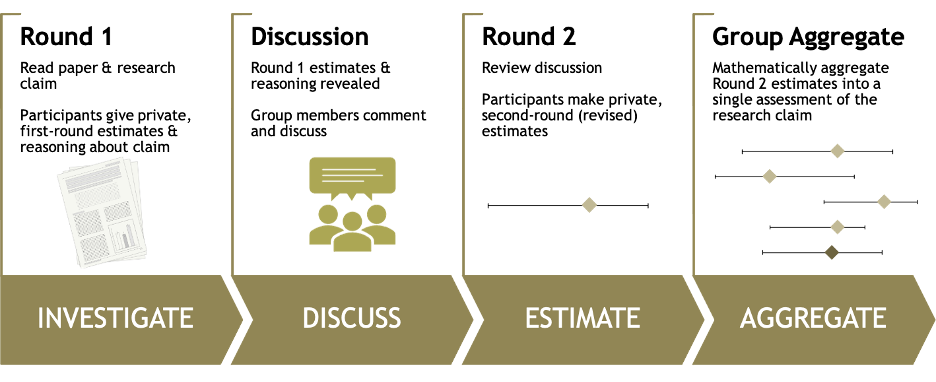
\includegraphics{images/img_IDEA_repliCATS.png}

}

\caption{The IDEA protocol as deployed by the repliCATS project
(reproduced with permission from Wintle et al. 2021).}

\end{figure}

\hypertarget{introducing-the-aggrecat-package}{%
\section{Introducing the aggreCAT
package}\label{introducing-the-aggrecat-package}}

In this paper we aim to provide a detailed overview of the
\pkg{aggreCAT} package so that researchers may apply the aggregation
functions described in \citep{Hanea2021} to their own expert elicitation
datasets where mathematical aggregation is required. Note that
judgements that have already been subjected to behavioural or consensus
aggregation may not be subsequently mathematically aggregated, however
individual elicited judgements may be aggregated mathematically as an
alternative or complement to behavioural or consensus-based aggregation.

We begin by formulating the problem of mathematically aggregating expert
judgements. Each method, and its data requirements is summarised in
Table \ref{tbl-method-summary-table}. Before outlining key aggregation
methods, we briefly summarise package datasets, which were collected by
the repliCATS project. By first describing the datasets before
describing the aggregation methods in detail, we aim to provide a
grounded understanding of the different outputs of expert elicitation
using the repliCATS IDEA protocol, and the inputs available to the
aggregation functions.

Next, we describe and illustrate the main types of aggregators, which
may be categorised according to their data requirements, mathematical
properties and computational implementation
(Section~\ref{sec-focal-claims}). By selecting representative functions
of each key aggregator type and applying them to a subset of focal
claims, we demonstrate the internal mechanics of how these methods
differently operationalise the data to generate forecasts or Confidence
Scores. We do not give advice on the circumstances in which each method
should be used, instead, choice of aggregation method should be informed
by the mathematical properties of the method, the desired properties of
an aggregation, and the purpose for which the aggregation is being used.
For a detailed description of each method as well as a discussion of
their relative merits, see \citep{Hanea2021}.

Finally, we provide a detailed workflow for aggregating expert judgments
for multiple forecasts, using multiple aggregation functions, as
implemented by the repliCATS project in the course of delivering \(>\)
4000 Confidence Scores for the DARPA SCORE program. The \pkg{aggreCAT}
package provides a set of supporting functions for evaluating or
ground-truthing aggregated forecasts or Confidence Scores against a set
of known-outcomes, as well as functions for visualising comparisons of
different aggregation methods and the outcomes of performance
evaluation. We describe and demonstrate this functionality in the
presentation of the repliCATS workflow. The workflow is representative
of the probable challenges faced by the researcher in the course of
mathematically aggregating groups of forecasts, and should equip the
reader to use \pkg{aggreCAT} for their own datasets; it exemplifies how
to extend the \pkg{aggreCAT} package to any expert judgement dataset
from any domain in which there are multiple judgements from multiple
individuals that must be combined into a single forecast.

\hypertarget{mathematically-aggregating-expert-judgements}{%
\section{Mathematically Aggregating Expert
Judgements}\label{mathematically-aggregating-expert-judgements}}

Mathematically, the aggregation methods can be divided into three main
types:

\begin{itemize}
\item
  Un-weighted linear combination of best estimates, transformed best
  estimates or distributions,
\item
  Weighted linear combinations of best estimates, transformed best
  estimates and of distributions, where weights are proxies of
  forecasting performance constructed from characteristics of
  participants and/or their judgements, and
\item
  Bayesian methods that use participant judgements as data with which to
  update both uninformative and informative priors.
\end{itemize}

However, the \pkg{aggreCAT} package user might wish to categorise the
aggregation methods according to aspects of their computational
implementation and data requirements, because these inform the function
arguments as well as the type and form of the data that is parsed to the
aggregation functions. These aspects include:

\begin{itemize}
\tightlist
\item
  Elicitation requirement, number of elicitation rounds: the majority of
  aggregation methods require data from only a single round of
  judgements, i.e.~the final post-discussion estimates. However, some
  aggregation methods require data from both rounds of judgements, which
  may be elicited using the IDEA protocol or other similar structured
  elicitation protocol in which there are two rounds of judgements.
\item
  Elicitation requirement, single point or three point elicitation:
  several aggregation methods use only a single data point elicited from
  individuals (their best estimate), however, most aggregation methods
  require a best estimate, and estimates of uncertainty in the form of
  upper and lower bounds.
\item
  Number of claims / forecasts assessed by the individual: some weighted
  aggregation methods consist of weights that are calculated from
  properties of participant judgements across multiple forecasting
  questions, not just the target claim being aggregation. Secondly, for
  aggregation methods that calculate variance in estimates, variance
  cannot be calculated on a single data point. While 2 is the
  mathematical minimum, the user should give consideration to what
  minimum number of claims should be used to reliably calculate measures
  of variance.
\item
  Supplementary data requirements: several aggregation methods require
  supplementary data collected either in addition to or as part of the
  repliCATS IDEA protocol, some of which will need additional
  qualitative coding before being parsed to the aggregation function.
\end{itemize}

The data and structured elicitation protocol requirements are described
in Table \ref{tbl-method-summary-table}. All aggregation methods
requiring a single round of estimates can therefore be applied to expert
judgments derived from any structured elicitation protocol that
generates, lower, upper, and best estimates from each individual
(i.e.~not just the IDEA protocol), and does not enforce behavioural
consensus.

\hypertarget{notation-and-problem-formulation}{%
\subsubsection{Notation and Problem
Formulation}\label{notation-and-problem-formulation}}

Here we describe some preliminary mathematical notation used to
represent each aggregation method. For the mathematical specification of
each individual aggregation function, please consult \citep{Hanea2021}
or the \pkg{aggreCAT} package function documentation.

The total number of research claims, \(claim\), or unique forecasts
being assessed, \(C\) , is indexed by \(c = 1, ..., C\). The total
number of individuals / experts / participants is denoted by \(N\), and
is indexed by \(i = 1, ..., N\). Each claim \emph{outcome} (i.e.~the
outcome of a replication study) assumes binary values, where the value
is 0 if the claim is false, and 1 if the claim is true. `\texttt{TRUE}'
claims are claims where the replication study found a significant result
in the same direction as the original research claim, and
`\texttt{FALSE}' claims are those where the replication study \emph{did
not} find a significant result in the same direction as the original
study. For each claim \(c\), an individual \(i\) assesses the
probability of a claim replicating by providing three probabilities: a
lower bound \({L}_{i,c}\), an upper bound \({U}_{i,c}\), and a best
estimate \(B_{i,c}\), satisfying the inequalities:
\(0 \le Li,c \le Bi,c \le Ui,c \le 1\).

Every claim is assessed by multiple individuals, and their probabilities
are aggregated using one of the aggregation methods to obtain a group or
aggregate probability, denoted by \(\hat{p}_c\). The aggregated
probability calculated using a specific method, is given by
\(\hat{p}_{c}\left(Method \space ID \right)\). Each aggregation is
assigned a unique \(Method \space ID\) which is the abbreviation of the
mathematical operation used in calculating the weights. Note that all
Best, Lower and Upper estimates are taken to be \texttt{round\ 2}
judgements from the repliCATS IDEA protocol
\protect\hyperlink{fig1}{Figure 1}), unless appended by a ``1'', where
they are \texttt{round\ 1} judgements, e.g.~\(B1_{i,c}\) denotes the
\texttt{round\ 1} Best estimate from individual \(i\) for claim \(c\).

\hypertarget{weighting-expert-forecasting-performance}{%
\paragraph{Weighting Expert Forecasting
Performance}\label{weighting-expert-forecasting-performance}}

Equal-weighting of judgements are less calibrated, accurate and
informative than weighted aggregation methods where judgements from
experts who performed well in similar judgement tasks are more heavily
weighted \citep{Hanea2021}. Proxies for forecasting performance, such as
breadth and variability of qualitative reasons used by experts to
justify their judgements, can be used to form weights in the absence of
measures of experts' prior performance \citep{Hanea2021}.

The aggregation methods other than the \fct{AverageWAgg} and Bayesian
approaches in \pkg{aggreCAT} each employ weighting schemes that are
informed by proxies for good forecasting performance whereby experts'
estimates are weighted differently by measures of reasoning, engagement,
openness to changing their mind in light of new facts, evidence or
opinions presented in the discussion round, extremity of estimates,
informativeness of estimates, asymmetry of estimate bounds, granularity
of estimates, and by prior statistical knowledge as measured in a quiz.

Below, we define standardised notation for describing weighted linear
combinations of individual judgements where un-normalised weights are
denoted by \(w\_method\) and normalised weights by
\(\tilde{w} \_ method\) (Equation~\ref{eq-eqn1}). Given that for all
aggregation methods weights are normalised, and that the normalisation
process is the same for each aggregation method, the equations for the
aggregation methods are presented for un-normalised weights.

\begin{equation}\protect\hypertarget{eq-eqn1}{}{
\hat{p}_c\left(Method \space ID \right) = \frac{1}{N}\sum_{i=1}^N \tilde{w}\_{method}_{i,c}  B_{i,c}
}\label{eq-eqn1}\end{equation}

By default, weights are calculated across all claims on a
per-individual, per-claim basis, such that judgements for the same
individual are weighted differently across all claims they have provided
judgements for. There are some exceptions to this default:
\texttt{GranWAgg}, \texttt{QuizWAgg}, \texttt{IndIntWAgg}
\texttt{IndIntAsymWAgg}, \texttt{VarIndIntWAgg}, \texttt{KitchSinkWAgg}.
Note that \texttt{IndIntWAgg,} and methods that include its weighting
function \texttt{weight\_nIndivInterval()} as a component, re-scale
weights by a fixed measure across all claims. Hence, for aggregation
methods that use information from multiple claims other than the target
claim for which the Confidence Score is being computed, each individual
claim \(c\) is indexed by \(d = 1, ..., C\). Where the default weighting
is used, this is coded into each function. However, where more complex
and method-specific weighting methods are used, modularised functions
have been created for ease of debugging. These function names are
prefixed with \texttt{weight\_}.

\hypertarget{package-datasets}{%
\subsection{Package datasets}\label{package-datasets}}

The \pkg{aggreCAT} package includes the core dataset
\texttt{data\_ratings} consisting of judgements elicited during a pilot
experiment exploring the performance of IDEA groups in assessing
replicability of a set of claims with ``known outcomes.''
``Known-outcome'' claims are SBS research claims that have been subject
to replication studies in previous large-scale replication
projects\footnote{Many labs 1, 2 and 3 \citet{Klein2014},
  \citet{Klein2018ManyL2}, \citet{Ebersole2016}, the Social Sciences
  Replication Project \citet{Camerer2018} and the Reproducibility
  Project Psychology \citet{aac4716}.}. Data were collected using the
repliCATS IDEA protocol at a two day workshop\footnote{See
  \citet{Hanea2021} for details. The workshop was held at the annual
  meeting of the Society for the Improvement of Psychological Science
  (SIPS),
  \href{https://osf.io/ndzpt/}{\textless https://osf.io/ndzpt/\textgreater{}}.}
in the Netherlands, on July 2019, at which 25 participants assessed the
replicability of 25 unique SBS claims. In addition to the probabilistic
estimates provided for each research claim assessed, participants were
also asked to rate the claim's plausibility and comprehensibility,
answer whether they were involved in any aspect of the original study,
and to provide their reasoning in support of their quantitative
estimates, which were used to form measures of reasoning breadth and
engagement \citep{Fraser:2021}.

\texttt{data\_ratings} is a \emph{tidy} \class{data.frame} wherein each
\emph{observation} (or row) corresponds to a single value in the set of
\texttt{value}s constituting a participant's complete assessment of a
research claim. Each research claim is assigned a unique
\texttt{paper\_id}, and each participant has a unique (and anonymous)
\texttt{user\_name}. The variable \texttt{round} denotes the round in
which each \texttt{value} was elicited (\texttt{round\_1} or
\texttt{round\_2}). \texttt{question} denotes the type of question the
\texttt{value} pertains to; \texttt{direct\_replication} for
probabilistic judgements about the replicability of the claim,
\texttt{belief\_binary} for participants' belief in the plausibility of
the claim, \texttt{comprehension} for participants' comprehensibility
ratings, and \texttt{involved\_binary} for involvement in the original
study. An additional column \texttt{element} maintains the tidy
structure of the data, while capturing the multiple \texttt{value}s that
comprise a full assessment of the replicability
(\texttt{direct\_replication}) of a claim; \texttt{three\_point\_best},
\texttt{three\_point\_lower} and \texttt{three\_point\_upper} denote the
best estimate and lower and upper bounds respectively.
\texttt{binary\_question} describes the \texttt{element} for both the
plausibility rating (\texttt{belief\_binary}) and involvement
(\texttt{involved\_binary}) questions, whereas \texttt{likert\_binary}
is the \texttt{element} describing a participant's
\texttt{comprehension} rating. Judgements are recorded in column
\texttt{value} in the form of percentage probabilities ranging from
(0,100). The \texttt{binary\_question}s corresponding to
comprehensibility and involvement consist of binary values (\texttt{1}
for the affirmative, and \texttt{-1} for the negative). Finally, values
corresponding to participants' comprehension ratings are on a
\texttt{likert\_binary} scale from \texttt{1} through \texttt{7}. Note
that additional columns with participant attributes can be included in
the ratings dataset if required by the user, we include the
\texttt{group} column in \texttt{data-ratings}, which describes the
group number the participant was a part of. Below we show some example
data for a single user for a single claim to illustrate this structure
of the core \texttt{data\_ratings} dataset.

\begin{verbatim}
R> options(width = 80)
R> library(tidyverse,quietly = TRUE)
R> library(aggreCAT)
R> aggreCAT::data_ratings %>% 
+  dplyr::filter(paper_id == dplyr::first(paper_id), 
+                user_name == dplyr::first(user_name)) %>% 
+  print(., n = nrow(.))
\end{verbatim}

\begin{verbatim}
# A tibble: 11 x 7
   round   paper_id user_name  question           element           value group
   <chr>   <chr>    <chr>      <chr>              <chr>             <dbl> <chr>
 1 round_1 100      fx3d4tmdhh direct_replication three_point_lower    30 UOM1 
 2 round_1 100      fx3d4tmdhh involved_binary    binary_question      -1 UOM1 
 3 round_1 100      fx3d4tmdhh belief_binary      binary_question      -1 UOM1 
 4 round_1 100      fx3d4tmdhh direct_replication three_point_best     40 UOM1 
 5 round_1 100      fx3d4tmdhh direct_replication three_point_upper    45 UOM1 
 6 round_1 100      fx3d4tmdhh comprehension      likert_binary         5 UOM1 
 7 round_2 100      fx3d4tmdhh comprehension      likert_binary         4 UOM1 
 8 round_2 100      fx3d4tmdhh belief_binary      binary_question      -1 UOM1 
 9 round_2 100      fx3d4tmdhh direct_replication three_point_lower    30 UOM1 
10 round_2 100      fx3d4tmdhh direct_replication three_point_upper    45 UOM1 
11 round_2 100      fx3d4tmdhh direct_replication three_point_best     39 UOM1 
\end{verbatim}

Not all data necessary for constructing weights on performance is
contained in \texttt{data\_ratings}. Additional data collected as part
of the repliCATS IDEA protocol are contained within separate datasets to
\texttt{data\_ratings}. Participants provided justifications for giving
particular judgemetns, and these are contained in
\texttt{data\_justifications}. On the repliCATS platform users were
given the option to comment on others' justifications
(\texttt{data\_comments}), to vote on others' comments
(\texttt{data\_comment\_ratings}) and on others' justifications
(\texttt{data\_justification\_ratings}). Finally, \pkg{aggreCAT}
contains three `supplementary' datasets containing data collected
externally to the repliCATS IDEA protocol: \texttt{data\_supp\_quiz},
\texttt{data\_supp\_priors}, and \texttt{data\_supp\_reasons}.

\hypertarget{sec-quiz-supplementary-data}{%
\subsubsection{Quiz Score Data}\label{sec-quiz-supplementary-data}}

Prior to the workshop, participants also completed an optional quiz on
statistical concepts and meta-research that we expect participants to be
aware of in order to reliably evaluate the replicability of research
claims. Quiz responses are contained in \texttt{data\_supp\_quiz} and
are used to construct performance weights for the aggregation method
\texttt{QuizWAgg} where each participant receives a \texttt{quiz\_score}
if they completed the quiz, and \texttt{NA} if they did not attempt the
quiz \citep[see][ for further details]{Hanea2021}.

\hypertarget{sec-reasonwagg-supplementary-data}{%
\subsubsection{Reasoning Data}\label{sec-reasonwagg-supplementary-data}}

\texttt{ReasonWAgg} uses the number of unique reasons given by
participants to support a Best Estimate for a given claim \(B_{i,c}\) to
construct performance weights, and is contained within
\texttt{data\_supp\_reasons}. Qualitative statements made by individuals
during claim evaluation were recorded on the repliCATS platform
\citep{Pearson2021} and coded as falling into one of 25 unique reasoning
categories by the repliCATS Reasoning team \citep{Wintle:2021}.
Reasoning categories include plausibility of the claim, effect size,
sample size, presence of a power analysis, transparency of reporting,
and journal reporting \citep{Hanea2021}. Within
\texttt{data\_supp\_reasons}, each of the reasoning categories that
passed our inter-coder reliability threshold are distributed as columns
in the dataset whose names are prefixed with \texttt{RW}, and for each
claim \texttt{paper\_id}, each participant \texttt{user\_id} is assigned
a logical \texttt{1} or \texttt{0} if they included that reasoning
category in support of their Best estimate for that claim. See
Section~\ref{sec-ReasoningWAgg} for details on the \texttt{ReasonWAgg}
aggregation method.

\hypertarget{sec-bayesian-supplementary-data}{%
\subsubsection{Bayesian Prior
Data}\label{sec-bayesian-supplementary-data}}

The method \texttt{BayPRIORsAgg} uses Bayesian updating to update a
prior probability of a claim replicating estimated from a predictive
model \citep{Gould2021a} using an aggregate of the best estimates for
all participants assessing a given claim \(c\) \citep{Hanea2021}. The
prior data is contained in \texttt{data\_supp\_priors} with each claim
in column \texttt{paper\_id} being assigned a prior probability (on the
logit scale) of the claim replicating in column \texttt{prior\_means}.

\hypertarget{aggregation-wrapper-functions}{%
\subsubsection{Aggregation Wrapper
Functions}\label{aggregation-wrapper-functions}}

Although there are 27 aggregation methods in total, we grouped methods
based on their mathematical properties into eight `wrapper' functions,
denoted by the suffix \texttt{WAgg}, the abbreviation of \emph{weighted
aggregation}: \texttt{LinearWAgg()}, \texttt{AverageWAgg()},
\texttt{BayesianWAgg()}, \texttt{IntervalWAgg()},
\texttt{ShiftingWAgg()}, \texttt{ReasoningWAgg()},
\texttt{DistributionWAgg()}, and \texttt{ExtremisationWAgg()}. The
specific aggregation \emph{method} is applied according to the
\texttt{type} argument, whose options are described in each aggregation
wrapper functions' help page.

\hypertarget{tidy-aggregation-and-prescribed-inputs}{%
\subsection{`Tidy' Aggregation and Prescribed
Inputs}\label{tidy-aggregation-and-prescribed-inputs}}

The design philosophy of \pkg{aggreCAT} is principled on `tidy' data
\citep{Wickham:2014vp}. Each aggregation method expects a
\class{data.frame} or \class{tibble} of judgements
(\texttt{data\_ratings}) as its input, and returns a \class{tibble}
consisting of the variables \texttt{method}, \texttt{paper\_id},
\texttt{cs} and \texttt{n\_experts} (see Section~\ref{sec-AverageWAgg}
for illustration of outputs); where \texttt{method} is a character
vector corresponding to the aggregation method name specified in the
\texttt{type} argument. Each aggregation is applied as a summary
function \citep{Wickham2017R}, and therefore returns a single row or
observation with a single confidence score \texttt{cs} for each claim or
\texttt{paper\_id}. The number of expert judgements summarised in the
aggregated confidence score is returned in the column
\texttt{n\_experts}. Because of the tidy nature of the aggregation
outputs, multiple aggregations can be applied to the same data with the
results of all aggregation methods row bound together in a single
\texttt{tibble}.

Each aggregation function requires values derived from three-point
elicitation (best-estimate, upper and lower bound), however, some
methods require only the best-estimates for mathematical aggregation.
For every aggregation function, the three-point elicitation values
corresponding to the \texttt{direct\_replication} question are required
inputs. Of the \texttt{question} and \texttt{element}s other than the
three-point elicitation \texttt{element}s belonging to the direct
replication \texttt{question}, only the \texttt{comprehension} question
with the \texttt{likert\_binary} elements is required -- this is an
input into {CompWAgg}, which is used to weight participants judgements.

\hypertarget{sec-focal-claims}{%
\section{Focal Claim Aggregation}\label{sec-focal-claims}}

We now demonstrate how judgements elicited from a diverse group of
individuals may be mathematically aggregated for a single forecasting
problem, using the datasets provided by \pkg{aggreCAT}. We illustrate
the internal mechanics of the weighting methods and the different data
requirements of each of the different types of aggregators -- namely;
methods with non-weighted linear combinations of judgements, weighted
linear combinations of judgements, re-scaled weighted linear
combinations of judgements, methods that require supplementary data, and
methods that require data elicited from the full IDEA protocol. Each
group of methods differs in the type of judgements elicited (single- or
three-point estimates), the number of elicitation rounds (one or two
rounds), whether multiple forecasts / elicited judgements are used
during confidence score computation for a target forecast / claim, and
finally whether supplementary data is required for aggregation.

Here we demonstrate the application of aggregation methods for each
group of methods using a set of `focal claims' selected from the pilot
study dataset supplied with the \pkg{aggreCAT} package. Below we subset
the dataset \texttt{data\_ratings} to include a sample of four claims
with judgements from five randomly-sampled participants. From these
focal claims, we select a target claim for which we will apply an
exemplar aggregation method from each mathematical aggregator
(Table~\ref{tbl-focal-claim} ).

\begin{verbatim}
R> set.seed(1234)
R> focal_claims <- data_ratings %>% 
+  dplyr::filter(paper_id %in% c("24", "138", "186", "108"))
R> # select 5 users to highlight in focal claim demonstration
R> focal_users <- focal_claims %>% 
+  dplyr::distinct(user_name) %>% 
+  dplyr::slice_sample(n=5)
R> # filter out non-focal users from focal claims
R> focal_claims <- focal_claims %>%  
+  dplyr::right_join(focal_users, by = "user_name") 
R> focal_claims
\end{verbatim}

\begin{verbatim}
# A tibble: 220 x 7
   round   paper_id user_name  question           element           value group
   <chr>   <chr>    <chr>      <chr>              <chr>             <dbl> <chr>
 1 round_1 108      15k6nbf8iz comprehension      likert_binary         7 UOM1 
 2 round_1 108      15k6nbf8iz direct_replication three_point_upper    90 UOM1 
 3 round_1 108      15k6nbf8iz direct_replication three_point_lower    40 UOM1 
 4 round_1 108      15k6nbf8iz belief_binary      binary_question       1 UOM1 
 5 round_1 108      15k6nbf8iz involved_binary    binary_question      -1 UOM1 
 6 round_1 108      15k6nbf8iz direct_replication three_point_best     65 UOM1 
 7 round_1 108      4680r67jsd direct_replication three_point_upper    60 UOM3 
 8 round_1 108      4680r67jsd direct_replication three_point_lower    40 UOM3 
 9 round_1 108      4680r67jsd direct_replication three_point_best     51 UOM3 
10 round_1 108      4680r67jsd comprehension      likert_binary         6 UOM3 
# ... with 210 more rows
\end{verbatim}

\hypertarget{tbl-focal-claim}{}
\begin{longtable}{rlrrr}

\toprule
Claim ID & User Name & Lower Bound & Best Estimate & Upper Bound \\ 
\midrule
108 & 05puszkipi & 50 & 60 & 70 \\ 
108 & 15k6nbf8iz & 40 & 65 & 90 \\ 
108 & 4680r67jsd & 60 & 80 & 90 \\ 
108 & mk1z46sqhr & 70 & 85 & 90 \\ 
108 & pjrkctyakp & 70 & 80 & 90 \\ 
\bottomrule
\caption{\label{tbl-focal-claim}Focal Claim Data: Round 2 expert judgements for claim 108 derived from a
subset of 5 claims and 5 participants from data~ratings. Judgements are
displayed as percentages. }\tabularnewline
\end{longtable}

\hypertarget{sec-AverageWAgg}{%
\subsection{Non-weighted linear combination of
judgements}\label{sec-AverageWAgg}}

We first demonstrate the mechanics of mathematical aggregation and its
implementation using the \pkg{aggreCAT} package with the simplest,
unweighted aggregation method, \texttt{ArMean}. All other aggregation
methods take this underlying computational blueprint, and expand on it
according to the aggregation methods' requirements (See
\protect\hyperlink{aggWorkflow}{Box 1} for details). \texttt{ArMean} (
Equation~\ref{eq-ArMean} ) takes the unweighted linear average
(i.e.~arithmetic mean) of the best estimates, \(B_{i,c}\).

\begin{equation}\protect\hypertarget{eq-ArMean}{}{
\hat{p}_c\left(ArMean \right ) = \frac{1}{N}\sum_{i=1}^N B_{i,c}
}\label{eq-ArMean}\end{equation}

Below we demonstrate the application of \texttt{ArMean} on a single
claim \texttt{108} for a subset of participants who assessed this claim.
We also illustrate this aggregation visually in
\protect\hyperlink{fig-ArMean}{Figure 2}. \texttt{ArMean} is applied
using the aggregation method \fct{AverageWAgg}, which is a wrapper
function for several aggregation methods that calculate different types
of averaged best-estimates (see \texttt{?AverageWAgg}). The function
returns the Confidence Score for the claim in the form of a
\class{tibble}:

\begin{verbatim}
R> focal_claims %>% 
+  dplyr::filter(paper_id == "108") %>%
+  AverageWAgg(type = "ArMean")
\end{verbatim}

\begin{verbatim}
# A tibble: 1 x 4
  method paper_id    cs n_experts
  <chr>  <chr>    <dbl>     <int>
1 ArMean 108         74         5
\end{verbatim}

\begin{figure}

{\centering 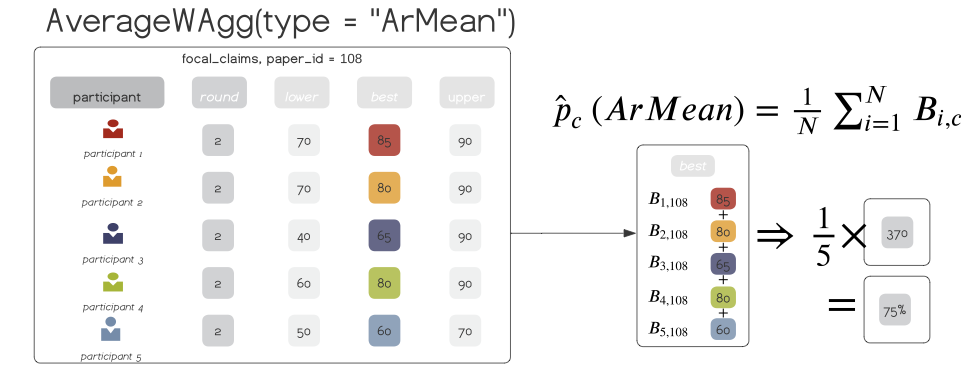
\includegraphics[width=3.26in,height=\textheight]{images/ArMean.png}

}

\caption{\label{fig-ArMean}ArMean with \texttt{AverageWAgg()} uses the
Estimates (shown in colour) from each participant to compute the mean.
We illustrate this using a single claim \texttt{108} for a subset of 5
out of 25 participants from the \texttt{data\_ratings} dataset. Note
that the data representations in this figure are for explanatory
purposes only, the data in the actual aggregation is tidy, with long
form structure and format.}

\end{figure}

\begin{tcolorbox}[enhanced jigsaw, arc=.35mm, breakable, colback=white, colframe=quarto-callout-color-frame, leftrule=.75mm, rightrule=.15mm, opacityback=0, bottomrule=.15mm, left=2mm, toprule=.15mm]

\hypertarget{aggWorkflow}{}
\hypertarget{box-1-aggregation-workflow-blueprint}{%
\subsection*{Box 1: Aggregation Workflow
Blueprint}\label{box-1-aggregation-workflow-blueprint}}
\addcontentsline{toc}{subsection}{Box 1: Aggregation Workflow Blueprint}

\hypertarget{argument-structure-and-expected-form}{%
\subsubsection{Argument Structure and Expected
Form}\label{argument-structure-and-expected-form}}

Each aggregation \emph{wrapper} function takes the following arguments:
\texttt{expert\_judgements}, \texttt{type}, \texttt{name},
\texttt{placeholder} and \texttt{percent\_toggle}:

\begin{verbatim}
R> args(AverageWAgg)
\end{verbatim}

\begin{verbatim}
function (expert_judgements, type = "ArMean", name = NULL, placeholder = FALSE, 
    percent_toggle = FALSE, round_2_filter = TRUE) 
NULL
\end{verbatim}

The aggregation \emph{method} to be applied by the aggregation
\emph{function}, is specified by the \texttt{type} argument, defaulting
to \texttt{ArMean} in the above example. The resultant \texttt{tibble}
of Confidence Scores includes the \texttt{name} of the aggregation
method applied, defaulting to the \texttt{type} argument, but this can
be overridden by the user if they supply a non-\texttt{NULL} value to
\texttt{name}. \textless br\textgreater{} Percentage values, counts, or
other non probabilistic quantities are the default expected value type
for ratings supplied to the \texttt{expert\_judgements} argument of
aggregation functions. By overriding the default value for the argument
\texttt{percent\_toggle} with \texttt{TRUE}, percentage values are
converted to probabilities by dividing judgements over 100 within the
aggregation functions.

When working with regularly updated data and developing a reproducible
pipeline \citep{Yenni2019} , it can be useful to put aggregation methods
into `placeholder' mode, whereby a placeholder value is returned by the
aggregation function instead of computing a Confidence Score using the
aggregation method. By setting \texttt{placeholder} to \texttt{TRUE},
the user can supply a placeholder Confidence Score, which defaults to
\(65\%\), the approximate average replication rate of SBS research
claims \citep{Camerer2018}. Should the user wish to set an alternative
value, they can create a modified version of
\texttt{method\_placeholder()} for themselves and store this within the
global environment. This function will then be called by the aggregation
method when the \texttt{placeholder} argument is set to \texttt{TRUE}.

Some functions expect additional arguments, especially those that rely
on additional or supplementary data. See the \emph{man} pages for
details of additional arguments.

\hypertarget{mathematical-aggregation-computational-workflow-blueprint}{%
\subsubsection{Mathematical Aggregation Computational Workflow
Blueprint}\label{mathematical-aggregation-computational-workflow-blueprint}}

Each aggregation function follows a general computational workflow
`blueprint' whereby the primary dataset \texttt{data\_ratings}, parsed
to the \texttt{expert\_judgements} argument, is first pre-processed by
\texttt{pre\_process\_judgements()}, weights are computed if applicable,
subsequently the aggregation method is applied using
\texttt{dplyr::summarise()}, and then finally the aggregated data is
parsed to \texttt{postprocess\_judgements()}.

The \texttt{preprocess\_judgements()} function parses the primary
dataset \texttt{data\_ratings} through the argument
\texttt{expert\_judgements} to filter the required quantitative inputs
for the aggregation method at hand. It uses two filtering arguments to
control which round of judgements are used as inputs
(\texttt{round\_2\_filter}), and whether the full set of three-point
elicitation judgements should be used, or whether other additional
elements must be returned (\texttt{three\_point\_filter}), including the
\texttt{likert\_binary} elements for participants' comprehensibility
ratings, and the plausibility ratings under \texttt{binary\_question} in
column \texttt{element}. \texttt{three\_point\_filter} defaults to
\texttt{TRUE} to provide only direct replication questions and
associated values. Nearly all aggregation functions use only the round 2
judgements, so the \texttt{round\_2\_filter} defaults to \texttt{TRUE}
(See Table \ref{tbl-method-summary-table} for required inputs of all
aggregation methods). \texttt{preprocess\_judgements()} further
pre-processes the data to remove missing data, and returnq the data into
an appropriate structure for calculating weights and applying the
aggregation function with \texttt{dplyr::summarise()}.

\begin{verbatim}
R> data_ratings %>% 
+  dplyr::group_by(paper_id) %>% 
+  tidyr::nest()  %>% 
+  dplyr::ungroup() %>% 
+  dplyr::slice_sample(n = 1) %>% 
+  tidyr::unnest(cols = c(data)) %>% 
+  preprocess_judgements() 
\end{verbatim}

\begin{verbatim}
\end{verbatim}

\begin{verbatim}
-- Pre-Processing Options --
\end{verbatim}

\begin{verbatim}
\end{verbatim}

\begin{verbatim}
i Round Filter: TRUE
\end{verbatim}

\begin{verbatim}
i Three Point Filter: TRUE
\end{verbatim}

\begin{verbatim}
i Percent Toggle: FALSE
\end{verbatim}

\begin{verbatim}
# A tibble: 75 x 5
   round   paper_id user_name  element           value
   <chr>   <chr>    <chr>      <chr>             <dbl>
 1 round_2 118      fx3d4tmdhh three_point_best     50
 2 round_2 118      fx3d4tmdhh three_point_upper    60
 3 round_2 118      fx3d4tmdhh three_point_lower    40
 4 round_2 118      sv2yl8jszy three_point_best     45
 5 round_2 118      sv2yl8jszy three_point_upper    70
 6 round_2 118      sv2yl8jszy three_point_lower    30
 7 round_2 118      v6n605nzv1 three_point_best     50
 8 round_2 118      v6n605nzv1 three_point_lower    40
 9 round_2 118      v6n605nzv1 three_point_upper    60
10 round_2 118      033t8xcqan three_point_best     64
# ... with 65 more rows
\end{verbatim}

The \texttt{preprocess\_judgements()} function is exposed to the user to
allow for data formatting in preparation for plotting, e.g.~with
\pkg{ggplot2} \citep{ggplot2016}, or for developing bespoke aggregation
functions / methods not supplied in \code{aggreCAT}.

For some aggregation methods, weights are necessary, and thus are
computed prior to aggregation. Some aggregation methods compute weights
using separate weighting functions (See Table
\ref{tbl-method-summary-table}), however, for aggregation methods with
simpler weight computations, these are defined in-function, rather than
being modularised.

After application of \texttt{preprocess\_judgements()}, weights are
constructed, and the aggregation method is applied, the function
\texttt{postprocess\_judgements()} then processes the variables into the
final data frame that is returned by each aggregation function. The post
processing function returns a \class{tibble} consisting of observations
equal to the number of unique claims that were parsed to
\texttt{postprocess\_judgements()}, the \texttt{method},
\texttt{paper\_id} , the Confidence Score \texttt{value}, as well as the
total number of participants \texttt{n\_experts} whose assessments were
used in the aggregation.

\end{tcolorbox}

\hypertarget{sec-IntWAgg}{%
\subsection{Weighted linear combinations of
judgements}\label{sec-IntWAgg}}

We now demonstrate the construction of weights for forecasting
performance, as well as the use of uncertainty bounds in addition to the
Best Estimates (i.e.~three-point estimates) in the aggregation
computation. The aggregation method \texttt{IntWAgg} weights each
participant's best estimate \(B_{i,c}\) by the width of their
uncertainty intervals, i.e.~the difference between an individual's upper
\({U}_{i,c}\) and lower bounds \({L}_{i,c}\). For a given claim \(c\), a
vector of weights for all individuals is calculated from their upper and
lower estimates using the weighting function, \fct{weight_interval},
which calculates the interval width for each individual's estimate for
the target claim. The weights are then normalised across the claim (by
dividing each weight by the sum of all weights per claim). Normalised
weights are then multiplied by the corresponding individual's best
estimates \(B_{i,c}\) andsummed together into a single Confidence Score
(Figure~\ref{fig-IntWAgg-IndIntWAgg}).

\hypertarget{re-scaled-weighted-linear-combinations-of-judgements}{%
\subsection{Re-scaled weighted linear combinations of
judgements}\label{re-scaled-weighted-linear-combinations-of-judgements}}

Individuals vary in the interval widths they give across different
claims. \texttt{IndIntWAgg} is a variation on \texttt{IntWAgg} that
accounts for cross-claim variation within individuals' assessments by
rescaling the interval width weights for individual \(i\) for claim
\(c\) relative to the widest interval provided by that individual across
all claims \(C\), (Equation~\ref{eq-IntWAgg}). For the target claim,
each individual's interval width is divided by the maximum interval
width that same individual gave across all claims they have provided
judgements for, using the weighting function \fct{weight_nIndivInterval}
(Equation~\ref{eq-weightnIndivInterval}). The process of re-scaling is
illustrated in Figure~\ref{fig-IntWAgg-IndIntWAgg}. Other aggregation
methods that re-scale weights by using data from multiple claims other
than the target claim under aggregation are \texttt{VarIndIntWAgg},
\texttt{IndIntAsymWAgg}, \texttt{KitchSinkWAgg} (applied with the
wrapper function \fct{IntervalWAgg}) and \texttt{GranWAgg} (applied with
the wrapper function \fct{LinearWAgg}), see Table
\ref{tbl-method-summary-table}.

\begin{equation}\protect\hypertarget{eq-weightnIndivInterval}{}{
w\_Interval_{i,c}= \frac{1}{U_{i,c} - L_{i,c}}
}\label{eq-weightnIndivInterval}\end{equation}

\begin{equation}\protect\hypertarget{eq-IntWAgg}{}{
\hat{p}_c\left( IntWAgg \right) = \sum_{i=1}^N \tilde{w}\_Interval_{i,c}B_{i,c}
}\label{eq-IntWAgg}\end{equation}

\newpage
\blandscape

\begin{figure}

{\centering 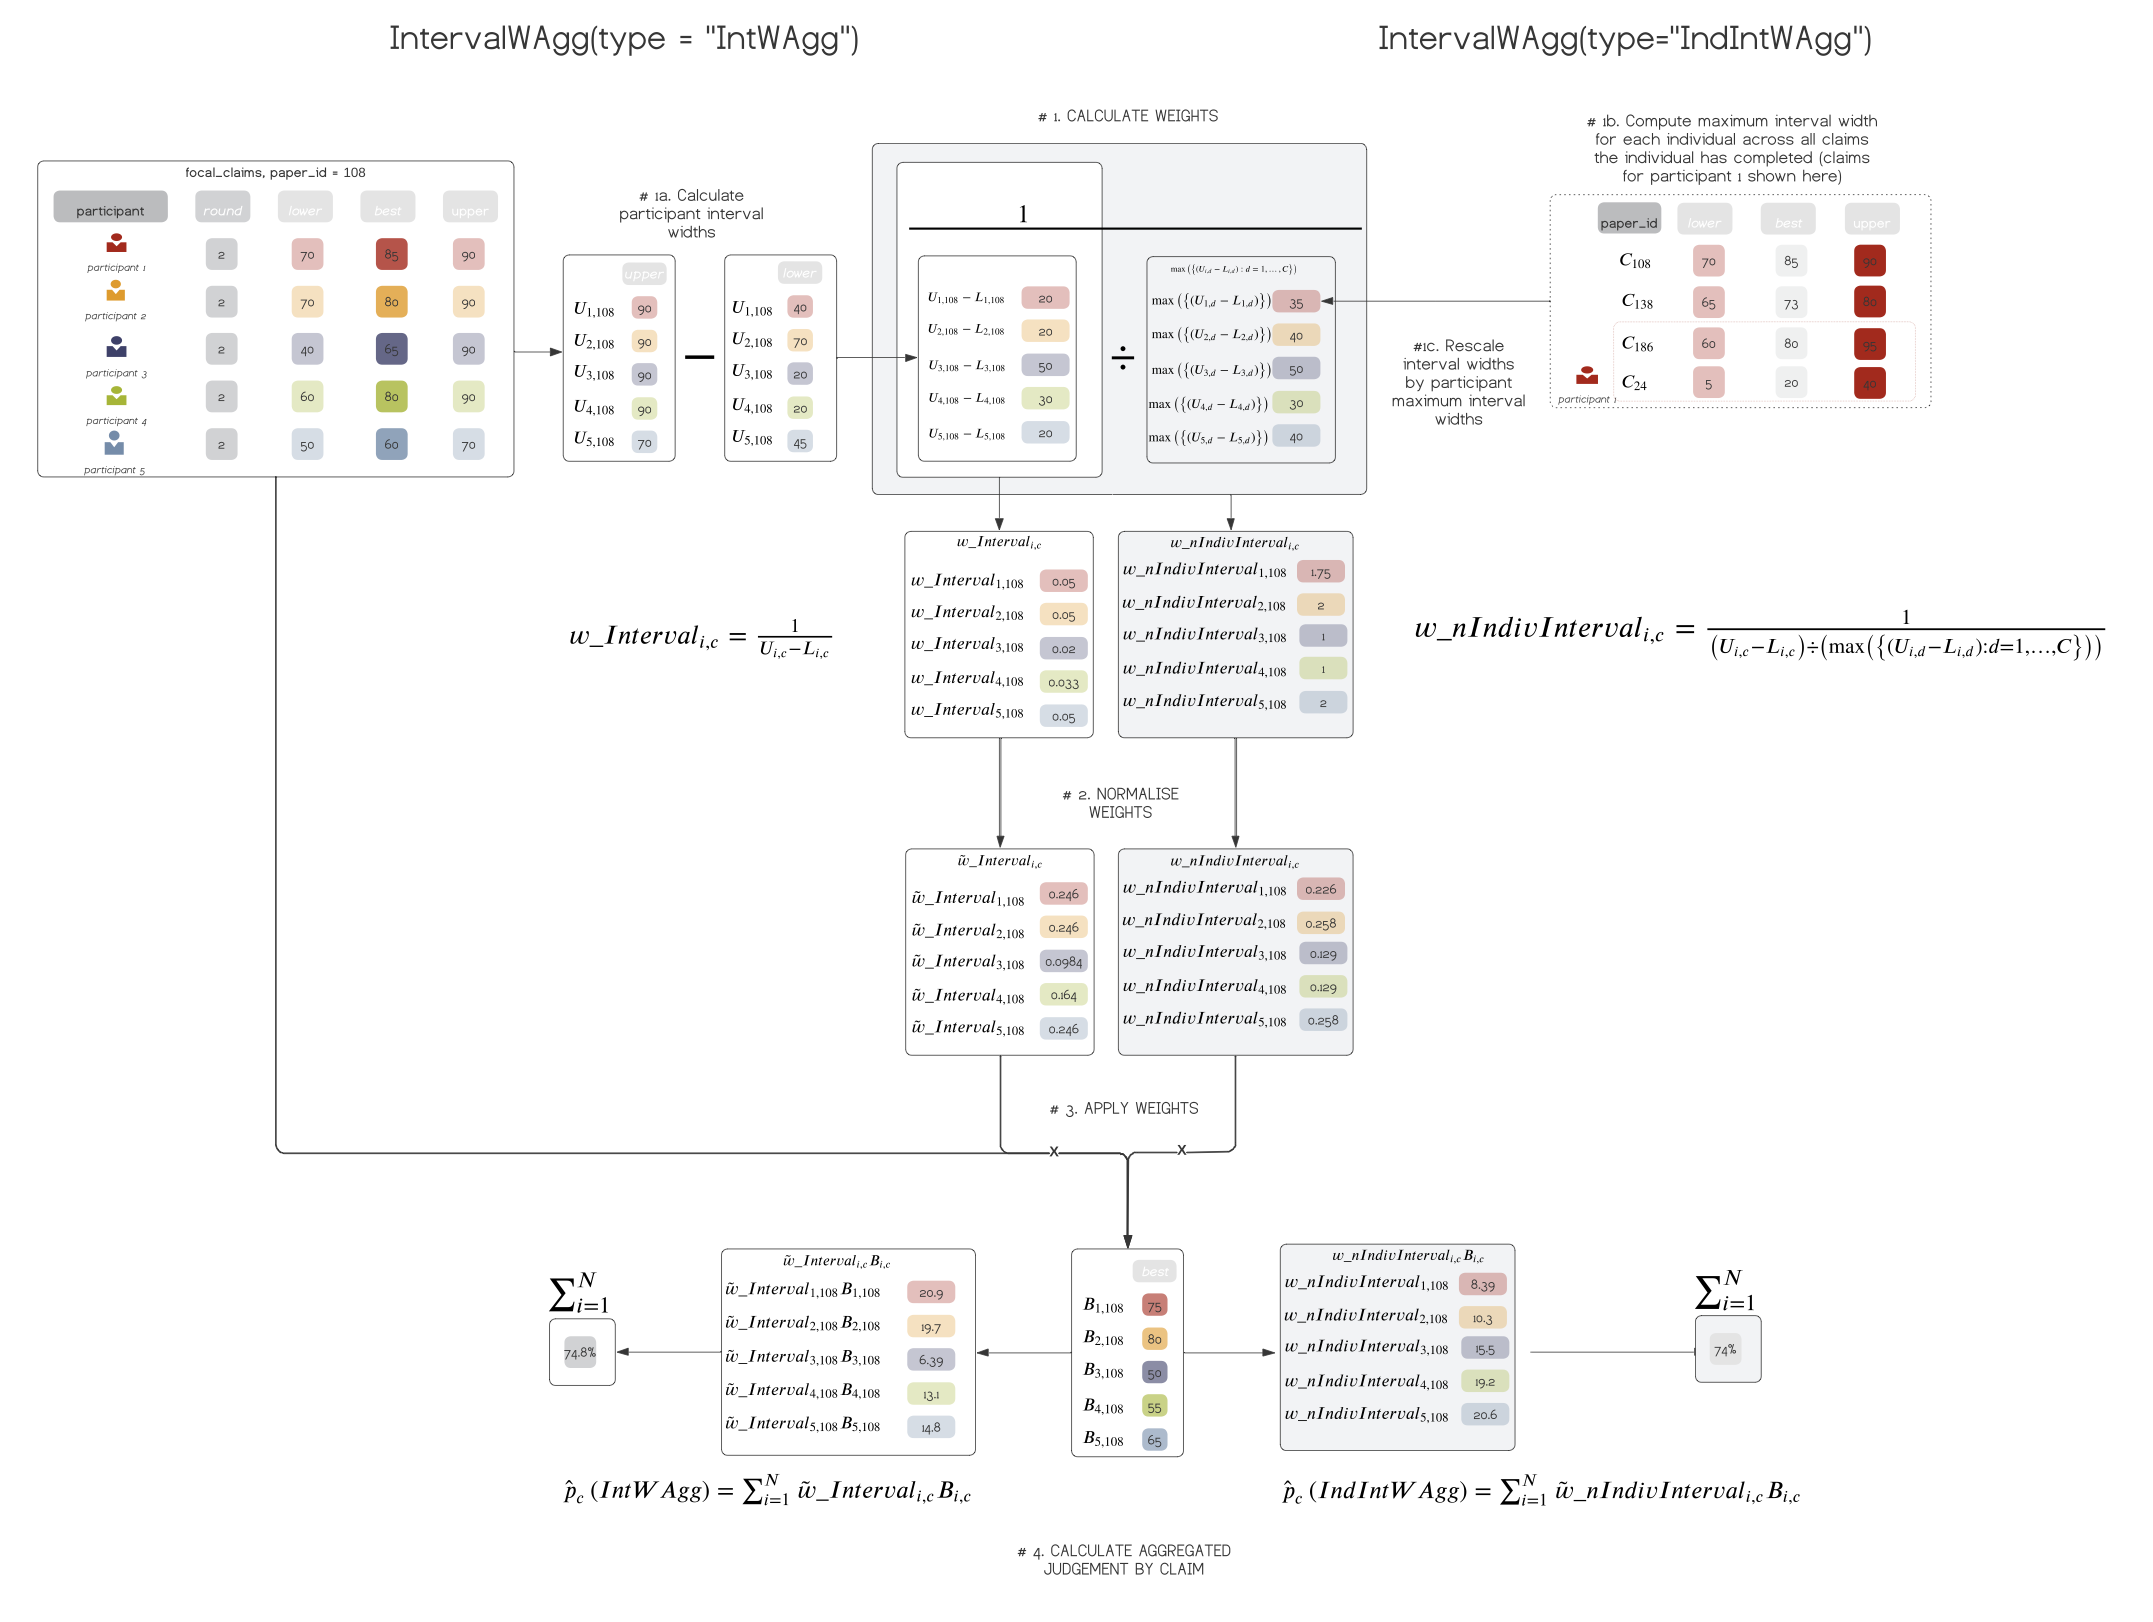
\includegraphics[width=7.18in,height=\textheight]{images/IntervalWAgg.png}

}

\caption{\label{fig-IntWAgg-IndIntWAgg}Example applications of
mathematical aggregation methods a) \texttt{IntWAgg} and b)
\texttt{IndIntWAgg} using the wrapper function a1) \texttt{IntWAgg} uses
participants' upper and lower bounds to construct performance weights.
b2) This weighting computation is modified in \texttt{IndIntWAgg}
whereby the weights for each individual are re-scaled by the largest
interval width across all claims for a given individual. We exemplify
this rescaling process by illustrating the calculation of participant
1's maximum interval width across all claims they assessed in the
demonstration dataset \texttt{focal\_claims}. This is repeated for every
individual who has assessed the target claim under aggregation.}

\end{figure}

\newpage
\elandscape

As for \fct{AverageWAgg}, when using the wrapper function
\fct{IntervalWAgg} we supply the aggregation method names as a character
vector to the \texttt{type} argument and the focal claim data frame to
the argument \texttt{expert\_judgements}, using \fct{dplyr::bind_rows}
to bind the resultant Confidence Scores together:

\begin{verbatim}
R> dplyr::bind_rows(
+  aggreCAT::IntervalWAgg(expert_judgements = focal_claims %>% 
+                           dplyr::filter(paper_id == "108"),
+                         type = "IndIntWAgg"),
+  aggreCAT::IntervalWAgg(expert_judgements = focal_claims %>% 
+                           dplyr::filter(paper_id == "108"),
+                         type = "IntWAgg")
+  )
\end{verbatim}

\begin{verbatim}
# A tibble: 2 x 4
  method     paper_id    cs n_experts
  <chr>      <chr>    <dbl>     <int>
1 IndIntWAgg 108       74           5
2 IntWAgg    108       74.8         5
\end{verbatim}

\hypertarget{sec-ReasoningWAgg}{%
\subsection{Aggregation Methods Requiring Supplementary
Data}\label{sec-ReasoningWAgg}}

In addition to the three-point elicitation dataset
\texttt{data\_ratings}, some aggregation methods require supplementary
data inputs collected externally to the repliCATS IDEA protocol. Each
aggregation wrapper function that requires supplementary data expects
this data to be provided as a \class{data.frame} or \class{tibble} in
addition to the main judgements that are provided to the
\texttt{expert\_judements} argument \ref{tbl-method-summary-table}.

We illustrate the usage and internal mechanics of this type of
aggregation with the method \texttt{ReasonWAgg}, which weights
participants' best estimates \(B_{i,c}\) by the breadth of reasoning
provided to support the individuals' estimate
(Equation~\ref{eq-ReasonWAgg}). This method is premised on the
expectation that multiple (unique) reasons justifying an individual's
judgement may indicate their breadth of thinking, understanding and
knowledge about both the claim and its context \citep{Hanea2021} while
also reflecting their level of engagement and general conscientiousness.
These qualities are correlated with improved forecasting
\citep{Wintle:2021}. Thus, greater weighting of best estimates that are
accompanied by a greater number of supporting reasons may yield more
reliable Confidence Scores.

\begin{equation}\protect\hypertarget{eq-ReasonWAgg}{}{
\hat{p}_c\left( ReasonWAgg \right) = \sum_{i=1}^N \tilde{w}\_reason_{i,c}B_{i,c}
}\label{eq-ReasonWAgg}\end{equation}

\texttt{ReasonWAgg} is applied with the wrapper function
\fct{ReasoningWAgg}, which uses the coded reasoning data
\texttt{data\_supp\_reasons}
(Section~\ref{sec-reasonwagg-supplementary-data}) to compute a vector of
weights, \(w\_reason_{i,c}\) , the number of unique reasons provided by
individual \(i\) in support of their estimate for claim \(c\)
(\protect\hyperlink{fig-ReasonWAgg}{Figure 4}). Weights are then
normalised across individuals, multiplied by the Best Estimates for that
claim \(B_{i,c}\) and weighted best estimates are then summed to
generate the Confidence Score (Equation~\ref{eq-ReasonWAgg}).

\begin{figure}

{\centering 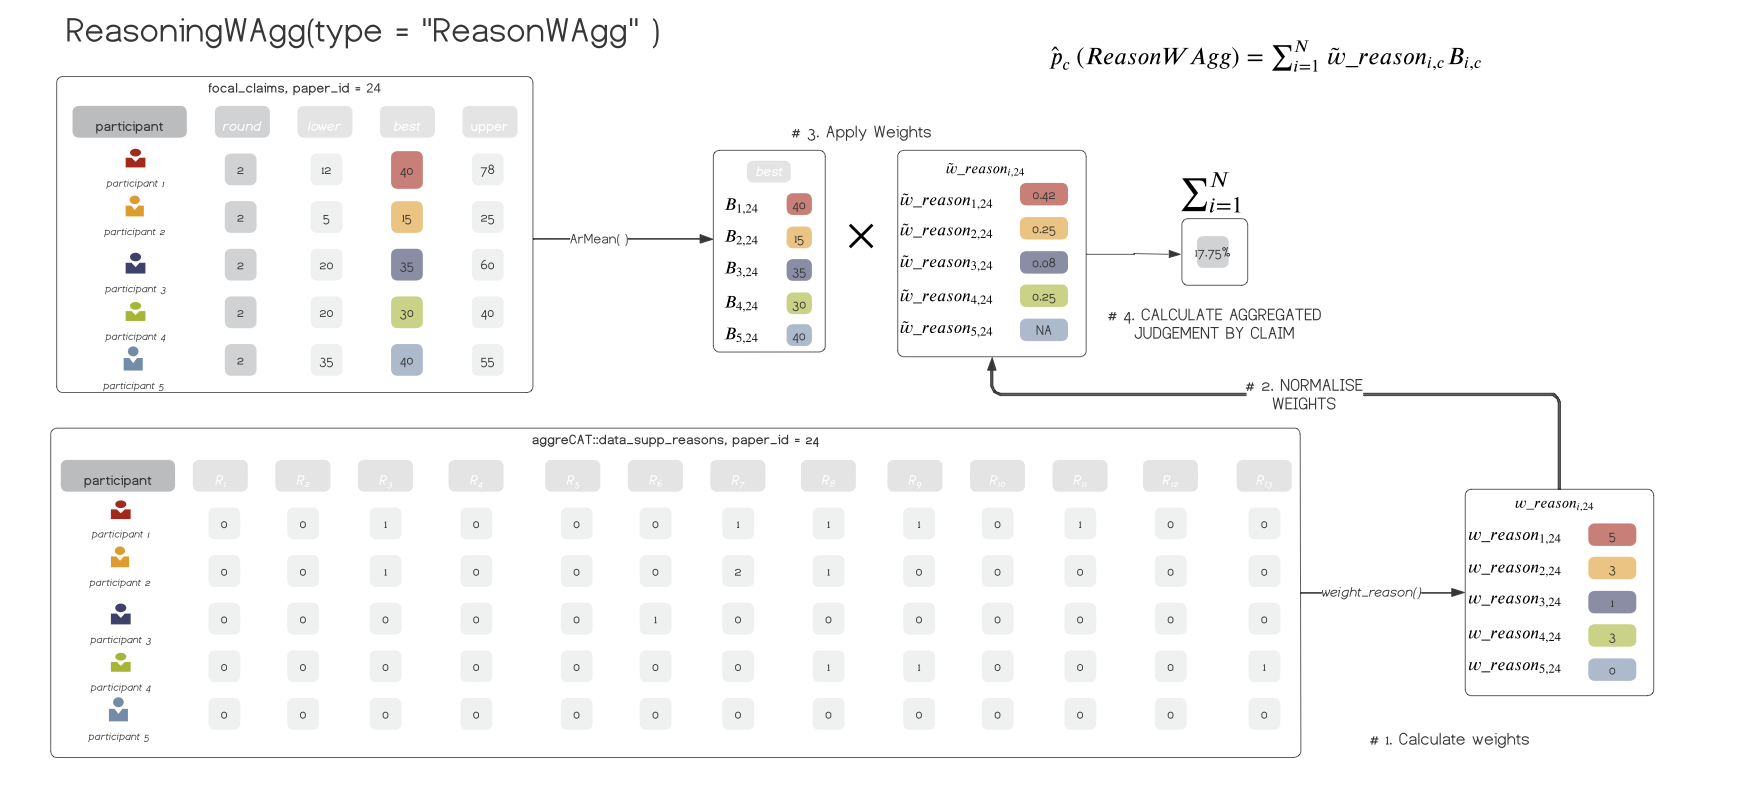
\includegraphics[width=5.82in,height=\textheight]{images/ReasonWAgg.png}

}

\caption{\label{fig-ReasonWAgg}Illustration of the \texttt{ReasonWAgg}
aggregation method for a subset of five participants who assessed claim
\texttt{24}. \texttt{ReasonWAgg} is applied using the wrapper function
\texttt{ReasoningWAgg()} and exemplifies aggregation methods that use
supplementary data (\texttt{data~supp~ReasonWAgg}) collected externally
to the IDEA protocol in the construction of weights and subsequent
calculation of Confidence Scores. Weights are constructed by taking the
sum of the number of unique reasons made in support of quantitative
estimates for each participant, for the target claim.}

\end{figure}

The focal claim selected for aggregation using \texttt{ReasonWAgg} is
\texttt{24}, the round two three-point estimates from the five focal
participants for this claim are shown in
Table~\ref{tbl-reason-wagg-focal-claim}. We first prepare the
supplementary data for aggregation \texttt{data\_supp\_reasons},
subsetting only the participants contained in our \texttt{focal\_claims}
dataset. We also illustrate a subset of the supplementary data for our
five focal participants for the focal claim \texttt{24} (see
\texttt{?data\_supp\_reasons} for a description of variables):

\begin{verbatim}
R> data_supp_reasons_focal <- aggreCAT::data_supp_reasons %>%  
+  dplyr::right_join(focal_users)
\end{verbatim}

\begin{verbatim}
Joining with `by = join_by(user_name)`
\end{verbatim}

\begin{verbatim}
R> data_supp_reasons_focal %>%
+  dplyr::filter( paper_id == 24) %>%
+  tidyr::pivot_longer(cols = c(-paper_id, -user_name)) %>%
+  dplyr::arrange(name) %>%
+  tidyr::separate(name, 
+                  into = c("reason_num", "reason"), 
+                  sep = "\\s", extra = "merge") %>%
+  dplyr::select(-reason) %>%
+  dplyr::group_by(paper_id, user_name) %>%
+  tidyr::pivot_wider(names_from = reason_num) %>%
+  dplyr::arrange(user_name)
\end{verbatim}

\begin{verbatim}
# A tibble: 5 x 15
# Groups:   paper_id, user_name [5]
  paper_id user_name  RW05  RW09  RW11  RW12  RW13  RW14  RW15  RW16  RW18  RW19
  <chr>    <chr>     <dbl> <dbl> <dbl> <dbl> <dbl> <dbl> <dbl> <dbl> <dbl> <dbl>
1 24       05puszki~     0     0     0     0     0     0     0     0     0     0
2 24       15k6nbf8~     0     0     0     0     0     1     0     0     0     0
3 24       4680r67j~     0     0     0     0     0     0     0     1     1     0
4 24       mk1z46sq~     0     0     1     0     0     0     1     1     1     0
5 24       pjrkctya~     0     0     1     0     0     0     2     1     0     0
# ... with 3 more variables: RW22 <dbl>, RW23 <dbl>, RW24 <dbl>
\end{verbatim}

\hypertarget{tbl-reason-wagg-focal-claim}{}
\begin{longtable}{rlrrr}

\toprule
Claim ID & User Name & Lower Bound & Best Estimate & Upper Bound \\ 
\midrule
24 & 05puszkipi & 35 & 40 & 55 \\ 
24 & 05puszkipi & 10 & 30 & 50 \\ 
24 & 15k6nbf8iz & 20 & 35 & 60 \\ 
24 & 15k6nbf8iz & 20 & 35 & 50 \\ 
24 & 4680r67jsd & 20 & 30 & 40 \\ 
24 & 4680r67jsd & 10 & 15 & 20 \\ 
24 & mk1z46sqhr & 12 & 40 & 78 \\ 
24 & mk1z46sqhr & 5 & 20 & 40 \\ 
24 & pjrkctyakp & 5 & 15 & 25 \\ 
24 & pjrkctyakp & 5 & 11 & 17 \\ 
\bottomrule
\caption{\label{tbl-reason-wagg-focal-claim}Focal Claim 24 judgements comprising best estimates, upper and lower
bounds elicited from five participants. Judgements are displayed as
percentages. }\tabularnewline
\end{longtable}

Confidence Scores estimating the replicability for claim \texttt{24}
(Table~\ref{tbl-reason-wagg-focal-claim}) using the \texttt{ReasonWAgg}
method are computed using \fct{ReasoningWAgg} and by providing the
supplementary data to the \texttt{reasons} argument:

\begin{verbatim}
R> focal_claims %>% 
+  dplyr::filter(paper_id == "24") %>% 
+  aggreCAT::ReasoningWAgg(reasons = data_supp_reasons_focal,
+                          type = "ReasonWAgg")
\end{verbatim}

Note that if there are zero participants with a Reasoning Score \(>0\)
or all participants are missing a Reasoning Score, the log-odds
transformed best estimate is returned instead (See
\texttt{?AverageWAgg}, \texttt{type="LOArMean"}). The user can choose to
flag this behaviour explicitly by setting the argument
\texttt{flag\_loarmean} to \texttt{TRUE}, which will generate new
columns in the aggregation output \class{data.frame} named
\texttt{method\_applied} (with values \texttt{LOArMean} or
\texttt{ReasonWAgg}), and \texttt{no\_reason\_score}, a logical variable
describing whether or not there were no reasoning scores for that claim.

\hypertarget{bayesian-aggregation-methods}{%
\subsection{Bayesian Aggregation
Methods}\label{bayesian-aggregation-methods}}

Both Bayesian methods \texttt{BayTriVar} and \texttt{BayPRIORsAgg} use
the full three-point elicitation data, i.e., they use information
contained in the uncertainty bound provided by individuals (upper
\({U}_{i,c}\) and lower bounds \({L}_{i,c}\)), in addition to Best
Estimates, \(B_{i,c}\). Like \texttt{IndIntWAgg} and other methods
(Table \ref{tbl-method-summary-table}), the Bayesian aggregation methods
also construct weights from information encoded in participant
assessments of claims other than the target claim under aggregation. In
fact, the Bayesian methods require more than a single claim's worth of
data to work properly execute due mathematical specification of the
models (See \texttt{?BayesianWAgg} and below for details).

The two Bayesian methods use the elicited probabilities as data to
update prior probabilities. \texttt{BayTriVar} incorporates three
sources of uncertainty in best estimates: variability in best estimates
across all claims, variability in estimates across all individuals, and
claim-participant variability (which is derived from an individuals'
upper and lower bounds). This Bayesian model, implemented using
\pkg{R2JAGS} \citep{R2JAGS}, takes the log odds transformed individual
best estimates, and uses a normal likelihood function to derive a
posterior distribution for the probability of replication. The estimated
confidence score is the mean of this posterior distribution.

\texttt{BayPRIORsAgg} is a modified version of \texttt{BayTriVar} where,
instead of using default priors, priors are generated from a predictive
model that estimates the probability of a claim replicating based on
characteristics of the claim and publication \citep{Gould2021a}. Priors
are parsed as supplementary data to the wrapper function
\fct{BayesianWAgg} using the argument \texttt{priors}
(Section~\ref{sec-bayesian-supplementary-data}) with each claim having
its own unique prior.

We illustrate aggregation of participant judgements using the method
\texttt{BayTriVar} to generate a Confidence Score for the claim
\texttt{108}. Note that \fct{BayesianWAgg} expects best estimates in the
form of probabilities, so to convert elicited values in the form of
percentages within the data parsed to \texttt{expert\_judgements} to
probabilities, the logical value \texttt{TRUE} is supplied to the
argument \texttt{percent\_toggle} (\protect\hyperlink{aggWorkflow}{Box
1}):

\begin{verbatim}
R> focal_claims %>% 
+  BayesianWAgg(type = "BayTriVar", 
+               percent_toggle = TRUE) %>% 
+  dplyr::filter(paper_id == "108")
\end{verbatim}

\begin{verbatim}
Compiling model graph
   Resolving undeclared variables
   Allocating nodes
Graph information:
   Observed stochastic nodes: 20
   Unobserved stochastic nodes: 4
   Total graph size: 230

Initializing model
\end{verbatim}

\begin{verbatim}
# A tibble: 1 x 4
  method    paper_id    cs n_experts
  <chr>     <chr>    <dbl>     <int>
1 BayTriVar 108      0.699         5
\end{verbatim}

The Confidence Score calculated for a given claim depends on data for
other claims and participants included in the
\texttt{expert\_judgements} argument other than the target claim,
because, by definition, \fct{BayesianWAgg} calculates the Confidence
Score for a target claim using data from participants' assessments of
other claims, and from all other claims in the \class{data.frame} parsed
to the \texttt{expert\_judgements} argument. Because information about
other claims than the target claim is used to calculate the Confidence
Score for the target claim, what is included in the data supplied to the
argument \texttt{expert\_judgements} in \fct{BayesianWAgg} will alter
the Confidence Score. Above, we calculated the Confidence Score for
claim \texttt{108} but including information from three additional
claims included in the \texttt{focal\_claims} \class{data.frame}:
\texttt{108}, \texttt{138}, \texttt{186}, \texttt{24}. However, if we
were to supply assessments for only two claims to \fct{BayesianWAgg},
then we would observe a different result for focal claim \texttt{108}:

\begin{verbatim}
R> focal_claims %>% 
+  dplyr::filter(paper_id %in% c("108", "138")) %>% 
+  aggreCAT::BayesianWAgg(type = "BayTriVar", percent_toggle = TRUE) %>% 
+  dplyr::filter(paper_id == "108")
\end{verbatim}

\begin{verbatim}
Compiling model graph
   Resolving undeclared variables
   Allocating nodes
Graph information:
   Observed stochastic nodes: 10
   Unobserved stochastic nodes: 2
   Total graph size: 116

Initializing model
\end{verbatim}

\begin{verbatim}
# A tibble: 1 x 4
  method    paper_id    cs n_experts
  <chr>     <chr>    <dbl>     <int>
1 BayTriVar 108      0.739         5
\end{verbatim}

The Confidence Score shifts from 0.7 to 0.74. Note that
\fct{BayesianWAgg} cannot calculate confidence scores when judgements
for only a single claim is provided to \fct{expert_judgements}, because
by definition the underlying Bayesian model calculates variance across
multiple claims and multiple participants:

\begin{verbatim}
R> focal_claims %>% 
+  dplyr::filter(paper_id == "108") %>% 
+  aggreCAT::BayesianWAgg(type = "BayTriVar", 
+                         percent_toggle = TRUE)
\end{verbatim}

\begin{verbatim}
Error in `aggreCAT::BayesianWAgg()`:
! Model requires n > 1 ids to successfully execute.
\end{verbatim}

Although we have set \(n=2\) as the minimum number of claims for which
variance is computed, it is up to the user to determine their own
justifiable minimum for reliable variance calculations.

Finally, all of the previous methods illustrated in this section have
been used with data generated using the IDEA elicitation protocol,
however this elicitation method is not strictly necessary for the of
these methods. Methods that \emph{do} require the full IDEA protocol for
their correct mathematical implementation, such as \fct{ShiftingWAgg},
which use two rounds of three-point judgements in which the second round
judgements are revised after discussion, are listed in Table
\ref{tbl-method-summary-table}.

\begin{figure}

{\centering 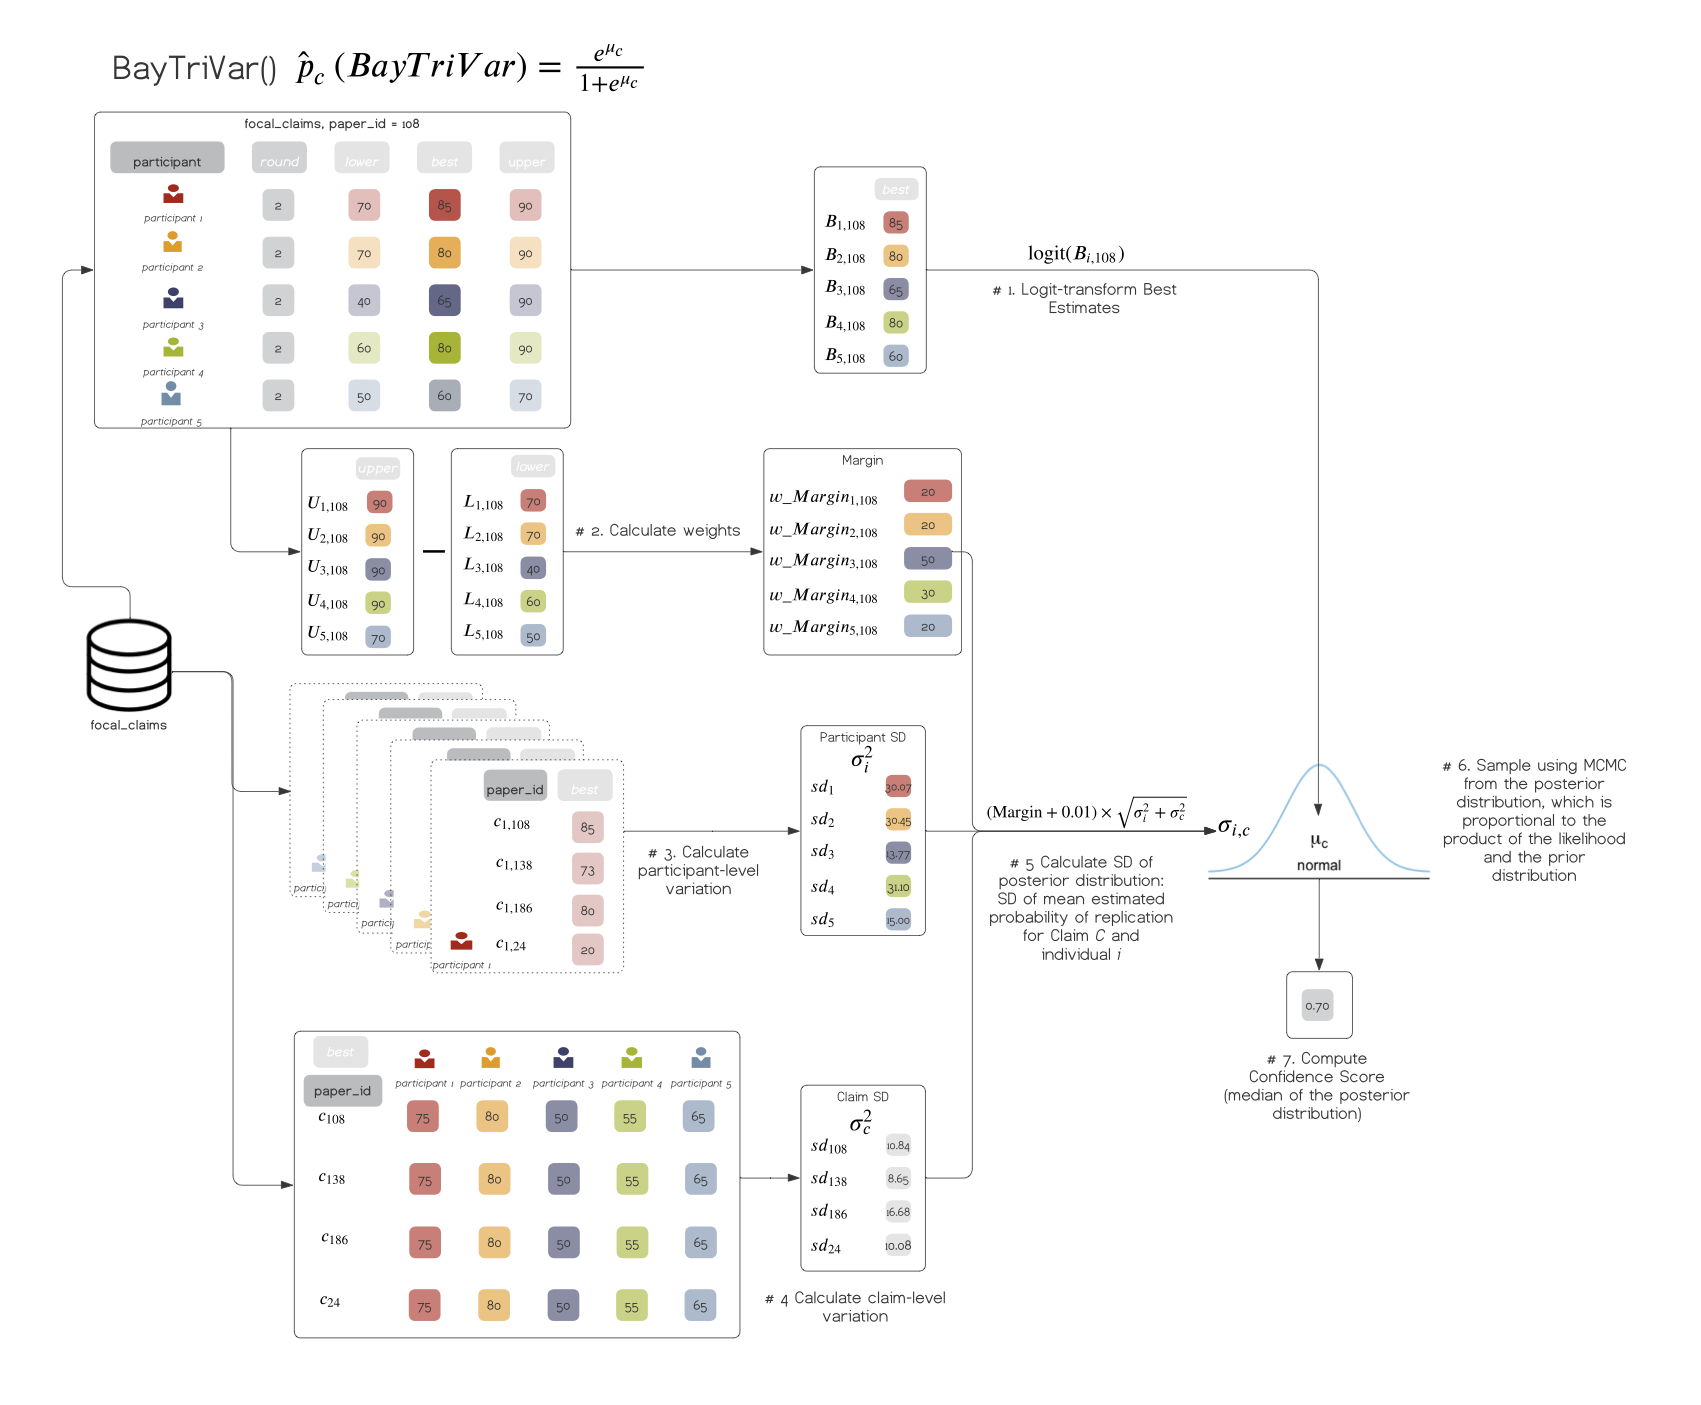
\includegraphics[width=5.67in,height=\textheight]{images/BayesianWAgg.png}

}

\caption{\label{fig-BayesianWAgg}Illustration of BayTriVar applied with
\texttt{BayesianWAgg()}for a single claim, \texttt{paper\_id\ =\ 108}
from the \texttt{focal\_claims} data object. Note that the claims
\texttt{138}, \texttt{186} and \texttt{24} contained in
\texttt{focal\_claims} are used in the calculation of pariticipant-level
SD and claim-level SD, thus the Confidence Score returned by BayTriVar
is sensitive to the other claims provided to argument
\texttt{expert\_judgements}.}

\end{figure}

\hypertarget{sec-workflow}{%
\section{An illustrative workflow for use in real study
contexts}\label{sec-workflow}}

Throughout the SCORE program, 752 participants assessed more than 4000
unique claims using the repliCATS IDEA protocol, between 7th July 2019
and 25 November 2021. This required batch aggregation over multiple
claims, and to generate Confidence Scores for multiple claims. We also
applied multiple aggregation methods to the same claim so that we could
compare and evaluate the different aggregation methods. We expect that
these are not uncommon use-cases,consequently in this section we
demonstrate a general workflow for using the \pkg{aggreCAT} package to
aggregate expert judgements using pilot data from DARPA SCORE program
generated by the repliCATS project.

\hypertarget{generating-multiple-forecasts}{%
\subsection{Generating multiple
forecasts}\label{generating-multiple-forecasts}}

During expert-elicitation the analyst or researcher may be tasked with
generating multiple forecasts for different problems or questions, and
therefore it is useful to batch the aggregation. Since the
\pkg{aggreCAT} package is designed using the principles of \emph{tidy}
data analysis \citep{tidyverse2019}, each aggregation function accepts a
\class{data.frame} of raw three-point forecasts for one or more claims,
\(C\), parsed to the argument \texttt{expert\_judgements}. The data
pre-processing and aggregation methods are applied using a combination
of calls to \pkg{tidyverse} functions, including \texttt{summarise} and
\texttt{mutate}. From the user's perspective, this means that data
processing and application of the aggergation methods is handled
internally by the \pkg{aggreCAT} package, rather than by the user. The
user is therefore free to focus their attention on the interpretation
and analysis of the forecasts. Here we demonstrate the application of
the \texttt{ArMean} aggregation method to four focal claims
simultaneously:

\begin{verbatim}
AverageWAgg(focal_claims, type = "ArMean")
\end{verbatim}

\begin{verbatim}
# A tibble: 4 x 4
  method paper_id    cs n_experts
  <chr>  <chr>    <dbl>     <int>
1 ArMean 108       74           5
2 ArMean 138       68.6         5
3 ArMean 186       57.6         5
4 ArMean 24        22.2         5
\end{verbatim}

\hypertarget{comparing-and-evaluating-aggregation-methods}{%
\subsection{Comparing and Evaluating Aggregation
Methods}\label{comparing-and-evaluating-aggregation-methods}}

In real study contexts, such as that of the repliCATS project in the
DARPA SCORE program, it is of interest to compute Confidence Scores
using multiple aggregation methods so that their performance might be
evaluated and compared. Since different methods offer different
mathematical properties, and therefore might be more or less appropriate
depending on the purpose of the aggregation and forecasting, a
researcher or analyst might want to check how the different assumptions
embedded in different aggregation methods influence the final Confidence
Scores for a forecast -- i.e.~how robust are the results to different
methods and therefore to different assumptions?

From a computational perspective, multiple aggregation methods must
first be applied to the forecast prior to comparison and evaluation.
This can be achieved by applying each different aggregation method to
\texttt{focal\_claims}, and binding the results together with
\pkg{dplyr}'s \fct{row_bind}. However, more elegant and succinct
solutions can be implemented using \pkg{purrr}'s \fct{map_dfr} function
\citep[see Listing~\ref{lst-multi-method-workflow-non-supp} and
Listing~\ref{lst-multi-method-workflow-both}]{purrr2020}.

\begin{verbatim}
R> confidenceSCOREs <- 
+  dplyr::bind_rows(
+    AverageWAgg(focal_claims,
+                "ArMean", 
+                percent_toggle = TRUE),
+    IntervalWAgg(focal_claims,
+                 "IndIntWAgg", 
+                 percent_toggle = TRUE),
+    IntervalWAgg(focal_claims,
+                 "IntWAgg", 
+                 percent_toggle = TRUE),
+    ShiftingWAgg(focal_claims,
+                 "ShiftWAgg", 
+                 percent_toggle = TRUE),
+    BayesianWAgg(focal_claims,
+                 "BayTriVar", 
+                 percent_toggle = TRUE),
+    ReasoningWAgg(aggreCAT::data_ratings, 
+                  reasons = aggreCAT::data_supp_reasons, 
+                  percent_toggle = TRUE)
+  )
\end{verbatim}

\begin{verbatim}
Compiling model graph
   Resolving undeclared variables
   Allocating nodes
Graph information:
   Observed stochastic nodes: 20
   Unobserved stochastic nodes: 4
   Total graph size: 230

Initializing model
\end{verbatim}

\begin{verbatim}
R> confidenceSCOREs
\end{verbatim}

\begin{verbatim}
# A tibble: 45 x 4
   method     paper_id    cs n_experts
   <chr>      <chr>    <dbl>     <int>
 1 ArMean     108      0.74          5
 2 ArMean     138      0.686         5
 3 ArMean     186      0.576         5
 4 ArMean     24       0.222         5
 5 IndIntWAgg 108      0.740         5
 6 IndIntWAgg 138      0.685         5
 7 IndIntWAgg 186      0.561         5
 8 IndIntWAgg 24       0.19          5
 9 IntWAgg    108      0.748         5
10 IntWAgg    138      0.694         5
# ... with 35 more rows
\end{verbatim}

After generating Confidence Scores using various aggregation methods, we
then evaluate the forecasts. We evaluated the repliCATS pilot study
forecasts against the outcomes of previous, high-powered replication
studies \citep{Hanea2021}, which are contained in the
\texttt{data\textbackslash{}\_outcomes} dataset published with
\pkg{aggreCAT}. In this dataset, each claim \texttt{paper\_id} is
assigned an \texttt{outcome} of \texttt{0} if the claim did not
replicate and \texttt{1} if the claim was successfully replicated:

\begin{verbatim}
R> aggreCAT::data_outcomes %>% 
+  head()
\end{verbatim}

\begin{verbatim}
# A tibble: 6 x 2
  paper_id outcome
  <chr>      <dbl>
1 100            1
2 102            0
3 103            0
4 104            1
5 106            0
6 108            1
\end{verbatim}

The function \fct{confidence_score_evaluation} evaluates a set of
aggregated forecasts or Confidence Scores against a set of known or
observed outcomes, returning the Area Under the ROC Curve (AUC), the
Brier score, and classification accuracy of each method
(Table~\ref{tbl-multi-method-workflow-eval}):

\hypertarget{tbl-multi-method-workflow-eval}{}
\begin{longtable}{lrrr}

\toprule
Method & AUC & Brier Score & Classification Accuracy \\ 
\midrule
ArMean & $1.00$ & $0.10$ & $100\%$ \\ 
BayTriVar & $1.00$ & $0.12$ & $100\%$ \\ 
IndIntWAgg & $1.00$ & $0.10$ & $100\%$ \\ 
IntWAgg & $1.00$ & $0.09$ & $100\%$ \\ 
ReasonWAgg & $0.90$ & $0.15$ & $84\%$ \\ 
ShiftWAgg & $1.00$ & $0.13$ & $75\%$ \\ 
\bottomrule
\caption{\label{tbl-multi-method-workflow-eval}AUC and Classification Accuracy for the aggregation methods `ShiftWAgg',
`ArMean', `IntWAgg', `IndIntWAgg', `ReasonWAgg' and `BayTriVar'
evaluated for repliCATS pilot study claims and known outcomes. }\tabularnewline
\end{longtable}

\hypertarget{visualising-judgements-confidence-scores-and-forecast-performance}{%
\subsection{Visualising Judgements, Confidence Scores and Forecast
Performance}\label{visualising-judgements-confidence-scores-and-forecast-performance}}

We include two functions for visualising comparison and evaluation of
Confidence Scores across multiple aggregation methods for a suite of
forecasts from multiple participants, \fct{confidence_scores_ridgeplot}
and \fct{confidencescore_heatmap}. \fct{confidence_scores_ridgeplot}
generates ridgeline plots using \pkg{ggridges} \citep{ggridges2021}, and
displays the distribution of predicted outcomes across a suite of
forecasts for each aggregation method, grouped into separate `mountain
ranges' according to the mathematical properties of the aggregation
method (Figure~\ref{fig-ridgeplot}).

\begin{figure}[H]

{\centering 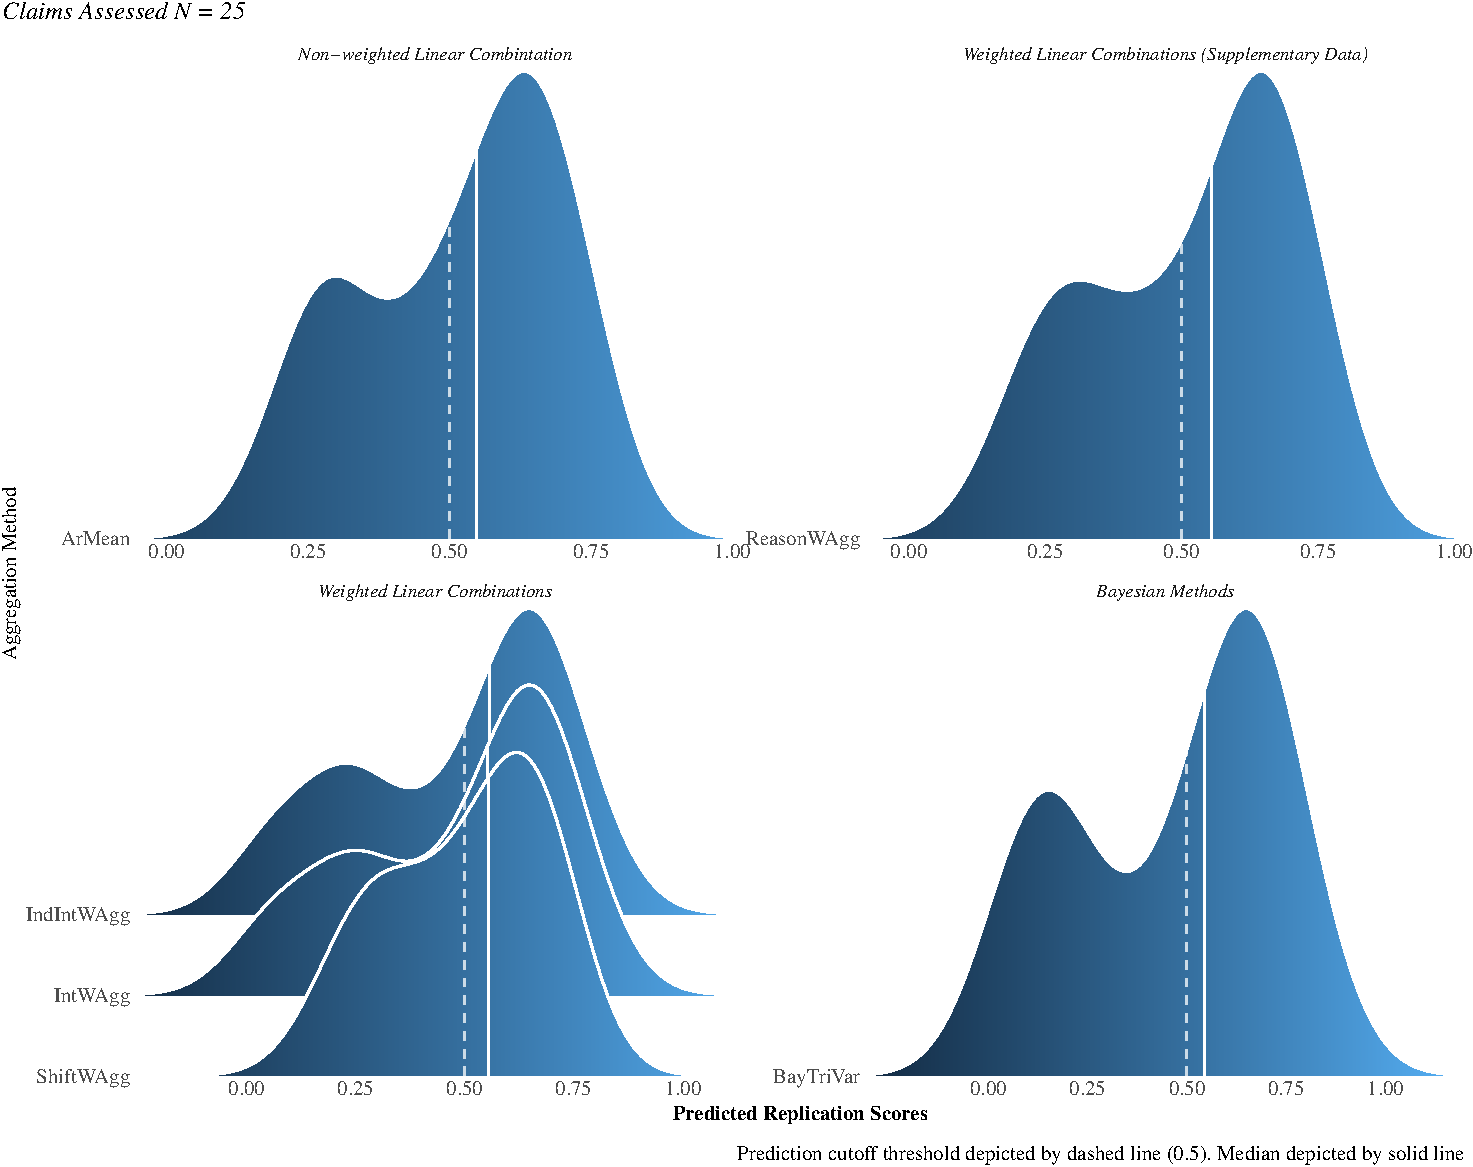
\includegraphics{aggreCAT_files/figure-pdf/fig-ridgeplot-1.pdf}

}

\caption{\label{fig-ridgeplot}Ridgeline plots illustrating the
distribution of aggregated Confidence Scores for the tibble
\texttt{confidenceSCOREs}, grouped according to mathematical properties
of each method.}

\end{figure}

\begin{figure}[H]

{\centering 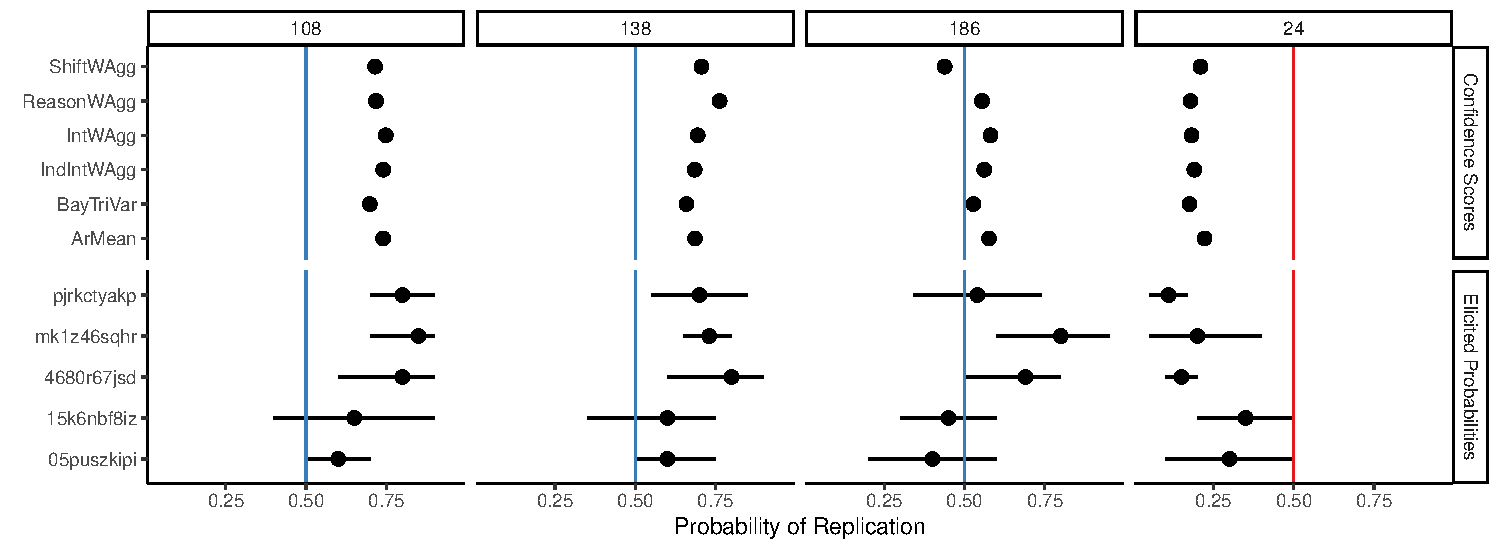
\includegraphics{aggreCAT_files/figure-pdf/fig-aggregation-1.pdf}

}

\caption{\label{fig-aggregation}Confidence Scores for the aggregation
methods \texttt{ArMean}, \texttt{BayTriVar}, \texttt{IntWAgg},
\texttt{IndIntWAgg}, \texttt{ReasonWAgg} and \texttt{ShiftWAgg} for four
claims. Participants' three-point best estimates are displayed as black
points, and their upper and lowr bounds displayed as black error bars.
Confidence Scores are displayed as points within the upper row of plots.
Lines are displayed vertically at the 0.5 probability mark, and their
colour denotes the observed outcome under previous large-scale
replication projects.}

\end{figure}

\begin{figure}[H]

{\centering 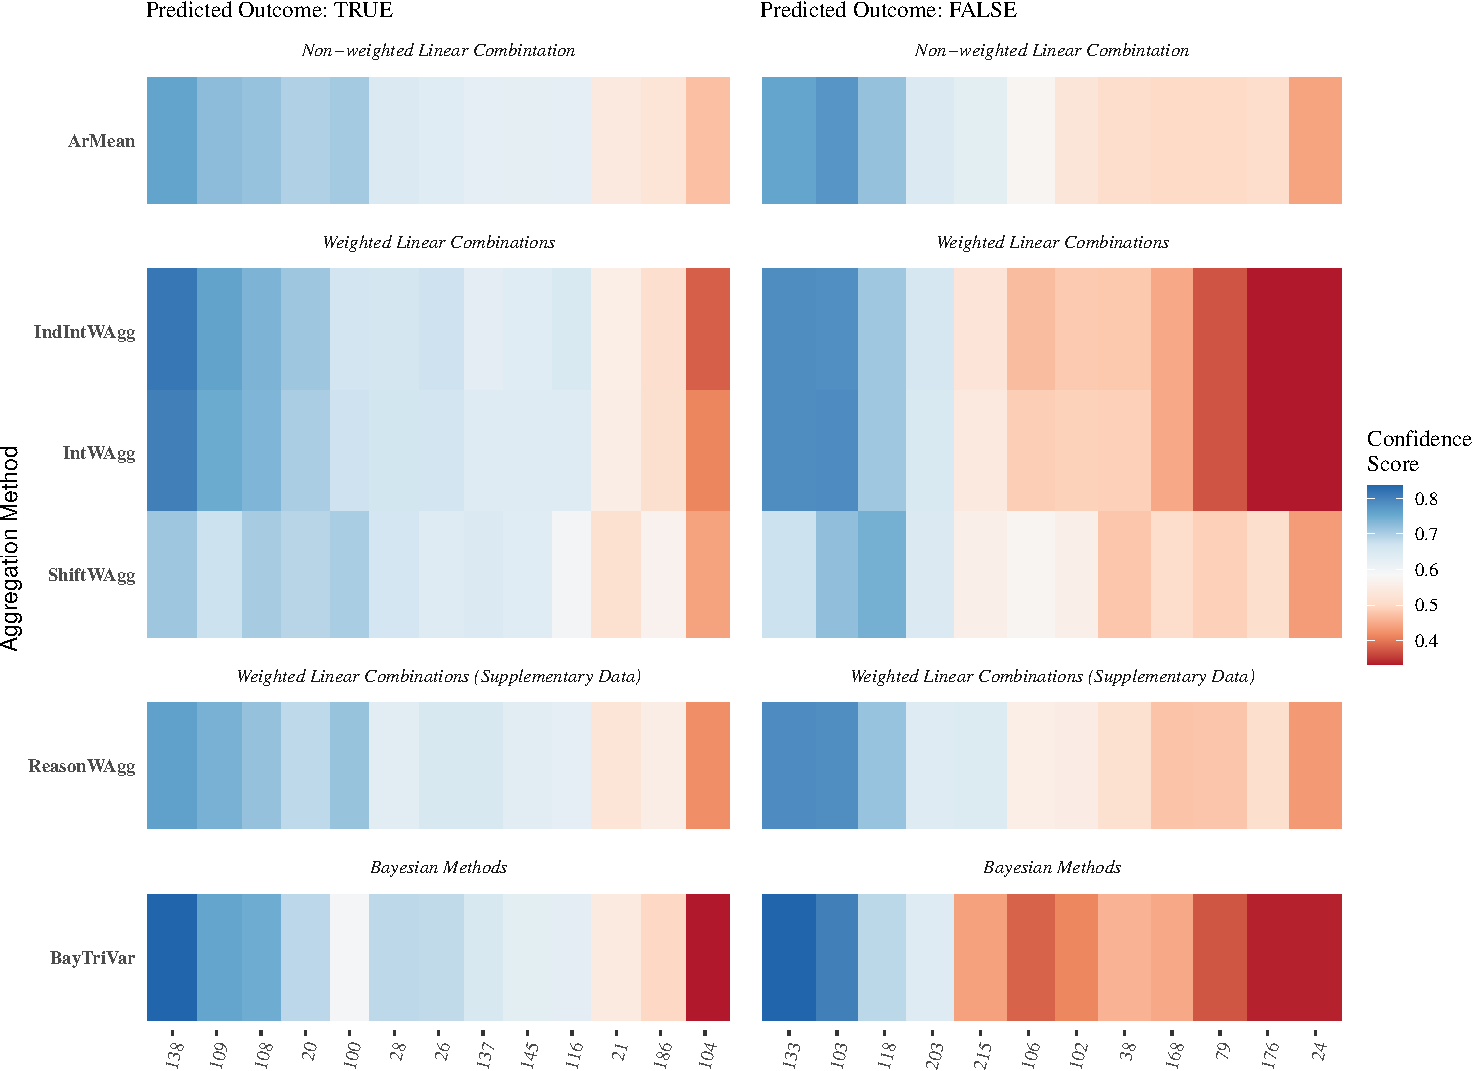
\includegraphics{aggreCAT_files/figure-pdf/fig-heatmap-1.pdf}

}

\caption{\label{fig-heatmap}Blocked heatmap visualisation of confidence
scores is useful for visually comparing aggregation methods and
evaluating them against a set of known outcomes. In this example,
Confidence Scores generated by six aggregation methods for the repliCATS
pilot study are visualised for 25 claims. Claims where known outcomes
succesfully replicated \texttt{outcome\ ==\ TRUE} are presented in
heatmap blocks on the left, and claims that failed to replicate are
presented in heatmap blocks on the right. Confidence Scores generated by
different aggregation methods are positioned along the y-axis, with
vertical groupings according to the methods' mathematical properties.
Colour and intensity of cells indicates the direction and degree of
deviation respectively of the Confidence Scores from the known
outcomes.}

\end{figure}

While \fct{confidencescore_heatmap} is useful for comparison of
aggregation methods, \fct{confidencescore_heatmap} is useful for visual
comparative \emph{evaluation} of aggregation methods.
\fct{confidencescore_heatmap} generates heatmaps of forecasted
Confidence Scores for each aggregation method included in the dataset
provided to the argument \texttt{confidence\_scores} organised with
unique aggregation methods on the y-axis, and separate forecasts or
\texttt{paper\_id}s along the y-axis (Figure~\ref{fig-heatmap}). The
heatmap is blocked vertically according to the mathematical
characteristics of each aggregation method, and horizontally into two
groups, according to the binary outcomes in \texttt{data\_outcomes}.

Horizontal grouping facilitates quick and simple evaluation of the
aggregation methods. Perfectly accurate aggregation methods show dark
blue squares in the left heatmap blocks, where the outcomes were
\texttt{1} or \texttt{TRUE}, and dark red squares on the right heatmap
blocks, where the actual outcomes were \texttt{0} or \texttt{FALSE}.
Deviation from this expectation indicates which aggregation methods for
which claim/forecast, for which outcome type were inaccurate, and to
what degree.

For example, in Figure~\ref{fig-heatmap}, for the example dataset
\texttt{confidenceSCOREs} the successful replication of most claims was
accurately forecasted by most methods, except for several claims. Some
methods performed better than others for some claims
(e.g.~\texttt{BayTriVar} and \texttt{IndIntWAgg} for the first claim on
the left (TODO insert), and for the claim on the right). In contrast,
for most claims that did not replicate, forecasts were inaccurate, with
\texttt{IndIntWAgg}, \texttt{IntWAgg} and \texttt{BayTriVar} performing
particularly badly for the claims X and Y.

Finally, creating bespoke user-defined plots is relatively easy --
because \pkg{aggreCAT} functions return tidy \class{data.frame}s or
\class{tibble}s, we can easily manipulate the raw judgements, aggregated
Confidence Scores and outcome data to plot them with \pkg{ggplot2}
\citep{ggplot2016} or other visualisation package. Below we plot the
aggregated Confidence Scores along with the three-point judgements
(subset using \fct{preprocess_judgements} on \texttt{focal\_claims},
transforming judgements in percentages to probabilities by setting
\texttt{percent\_toggle} to \texttt{TRUE}, Figure~\ref{fig-aggregation},
Listing~\ref{lst-confidencescores}).

\hypertarget{extending-aggrecat-to-other-datasets}{%
\subsection{Extending aggreCAT to other
datasets}\label{extending-aggrecat-to-other-datasets}}

The aggregation methods supplied by the \pkg{aggreCAT} package can
easily be applied to other forecasting problems. The only requirements
are that the data inputs adhere to the required format (Box
\protect\hyperlink{aggWorkflow}{1}), and that the expert judgements are
elicited using the appropriate method, as required by each aggregation
method (see Table \ref{tbl-method-summary-table}).

Judgement data provided to the \texttt{expert\_judgements},
\texttt{data\_justifications} or any supplementary data inputs argument
must contain the requisite column names, and be of the correct data
type, as described in each method's documentation (see
\texttt{?data\_ratings}, for example). At minimum the user must supply
to \texttt{expert\_judgements}: the \texttt{round} under which each
judgement is elicited, a unique ID for each different forecasting
problem \texttt{paper\_id}, a unique \texttt{user\_name} for each
individual, and the \texttt{element} of the three point elicitation that
the recorded response or \texttt{value} in that row corresponds to. The
data is stored in long or tidy format such that each row or observation
in the \class{data.frame} references only a single \texttt{element} of a
participants' set of three point elicitation values. When applying
aggregation methods requiring supplementary data to the elicitation
data, the analyst should also adhere to the requirements stipulated for
the relevant supplementary dataset described in the documentation.

Although several aggregation methods \emph{require} judgements that are
elicited using the IDEA protocol (See Table
\ref{tbl-method-summary-table} for exceptions), most aggregation methods
require only a single round of elicitation that generates a set of three
points; a best estimate, and upper and lower bounds about those
estimates, even if the IDEA protocol was used to elicit judgements.
Hence, the aggregation functions contained in the \pkg{aggreCAT} package
are unsuitable for use with judgements elicited with methods that
aggregate behaviourally (e.g.~using consensus) and therefore result in a
single forecast value. Where the analyst elicits judgements for only a
single round, the analyst should record the round in the judgements data
as the character string \texttt{"round\_1"}, and set the
\texttt{round\_2\_filter} argument to \texttt{FALSE} in the aggregation
wrapper function call.

Should the analyst wish to create their own aggregation functions, pre-
and post-processing functions may be leveraged inside the functions
(\fct{preprocess_judgements} and \fct{postprocess_judgements},
respectively), as we have illustrated in data preparation for
Figure~\ref{fig-aggregation} (Listing~\ref{lst-confidencescores}). These
processing functions modularise key components of the aggregation's
computational implementation -- namely the data wrangling that occurs
before and after the actual mathematical aggregation.

\hypertarget{preparing-your-own-elicitation-data}{%
\subsubsection{Preparing your own Elicitation
Data}\label{preparing-your-own-elicitation-data}}

We demonstrate how to prepare data for applying the \pkg{aggreCAT}
aggregation methods with data collected using the IDEA protocol for an
environmental conservation problem \citep{Arlidge2020} . Participants
were asked ``How many green turtles in winter per month would be saved
using a total gillnet ban, with gear switching to lobster potting or
hand line fishing required?''. We take the required data for the
\texttt{expert\_judgements} argument from Table S51 of Arlidge et al.
\citeyearpar{Arlidge2020}, make the data long instead of wide, and then
add the required additional columns \texttt{paper\_id} and
\texttt{question}:

\begin{verbatim}
R> green_turtles <- 
+  dplyr::tribble(~user_name, ~round, ~three_point_lower, 
+          ~three_point_upper, ~three_point_best,
+          "L01", 1,    10.00,  16.43,  10.00,
+          "L01", 2,    10.00,  16.43,  10.00,
+          "L02", 1,    500.00, 522.50, 500.00,
+          "L02", 2,    293.75, 406.25, 350.00,
+          "L03", 1,    400.00, 512.50, 400.00,
+          "L03", 2,    300.00, 356.25, 300.00,
+          "L04", 1,    32.29,  65.10,  41.67,
+          "L04", 2,    32.29,  65.10,  41.67,
+          "L05", 1,    6.67,   7.74,   6.67,
+          "L05", 2,    6.67,   7.74,   6.67) %>% 
+  dplyr::group_by(user_name) %>% # pivot longer
+  tidyr::pivot_longer(cols = tidyr::contains("three_point"), 
+               names_to = "element", values_to = "value") %>% 
+  dplyr::mutate(paper_id = 1, 
+         round = ifelse(round ==1, "round_1", "round_2"),
+         question = "direct_replication")
\end{verbatim}

We can then apply multiple aggregation methods, using the same approach
implemented for aggregation of the \texttt{focal\_claims} dataset
(Listing~\ref{lst-BYO-data-aggregate}), with aggregated Confidence
Scores shown in Table~\ref{tbl-BYO-data-aggregate}. Note that because
the judgements are absolute values rather than probabilities, we set the
\texttt{percent\_toggle} argument for each aggregation wrapper function
to {FALSE} (Listing~\ref{lst-BYO-data-aggregate}).

\hypertarget{tbl-BYO-data-aggregate}{}
\begin{longtable}{lrrr}

\toprule
Method & Question ID & Confidence Score & N (experts) \\ 
\midrule
ArMean & 1 & $141.67$ & 5 \\ 
IndIntWAgg & 1 & $141.67$ & 5 \\ 
IntWAgg & 1 & $15.26$ & 5 \\ 
ShiftWAgg & 1 & $328.85$ & 5 \\ 
\bottomrule
\caption{\label{tbl-BYO-data-aggregate}Example aggregation of non-percentage / non-probabilistic estimates with
several aggregation methods using Green Turtle dataset (Arlidge et al.
2020). }\tabularnewline
\end{longtable}

\hypertarget{sec-summary}{%
\section{Summary and Discussion}\label{sec-summary}}

The \pkg{aggreCAT} package provides a diverse suite of methods for
mathematically aggregating judgements elicited from groups of experts
using structured elicitation procedures, such as the IDEA protocol. The
\pkg{aggreCAT} package was developed by the repliCATS project as a part
of the DARPA SCORE program to implement the 27 aggregation methods
described in Hanea et al. \citeyearpar{Hanea2021}.

There are very few open-source tools available to the researcher wishing
to mathematically aggregate judgements. The \pkg{aggreCAT} package is
therefore unique in both the diversity of aggregation methods it
contains, as well as in its computational approach to implementing the
aggregation methods. There is no other R or other software package with
so many aggregation methods, and methods that use proxies of forecasting
accuracy using weights.

The \pkg{aggreCAT} package is production-ready for application to data
elicited during either a single workshop, or for contexts where data
collection may be ongoing and continuous analysis is used for automating
aggregation. Unlike other aggregation packages, the \pkg{aggreCAT}
package is designed to work within the \emph{tidyverse}. The package is
premised on the principles of \emph{tidy} data analysis whereby the user
supplies \class{data.frame}s of elicited judgements, and the aggregation
methods return \class{data.frame}s of aggregated forecasts. The benefits
of this approach are three-fold. Firstly, the work of data-wrangling and
application of the aggregation methods is handled internally by the
aggregation methods, so that the researcher can focus on analysis and
interpretation of the aggregation outputs. This is critical in
data-deficient contexts where rapid assessments are needed, which is a
common use-case for the use of expert derived forecasts. Secondly, the
\pkg{aggreCAT} package is easily paired with other tidyverse tools, such
as \pkg{purrr}, \pkg{dplyr}, and \pkg{ggplot2}, as exemplified through
the repliCATS workflow described in Section~\ref{sec-workflow}.

Thirdly, application of the \pkg{aggreCAT} package aggregation methods
and performance evaluation tools is scalable, which is evidenced by the
application of the \pkg{aggreCAT} package to forecast the replicability
of over 4000 research claims by the repliCATS project. The scalability
and placeholder functionality allow the \pkg{aggreCAT} package to be
built into production-ready pipelines for more complicated analyses
where there are multiple forecasts being elicited and aggregated, where
there are numerous participants, and where multiple aggregation methods
are applied.

Finally, through the provision of built-in performance metrics, the
analyst is able to `ground-truth' and evaluate the forecasts against
known-outcomes, or alternative forecasting methods
\citep[e.g.][]{Arlidge2020}.

The \pkg{aggreCAT} package is easily extensible and production-ready.
Each aggregation function follows a consistent modular blueprint,
wherein data-wrangling of the inputs and outputs of aggregation is
largely handled by pre- and post-processing functions
(\fct{preprocess_judgements} and \fct{postprocess_judgements},
respectively). This design expedites debugging by making it easier to
pinpoint the exact source of errors, while also permitting the user to
easily create their own custom aggregation methods.

Although the package currently requires data inputs to conform to
nomenclature specific to the repliCATS project, future releases of the
\pkg{aggreCAT} package will relax the data-input requirements so they
are more domain-agnostic. We believe this to be a minimal barrier for
adoption and application of the \pkg{aggreCAT} package. Ecologists
should be no stranger to these naming conventions for data requirements,
with packages like \pkg{vegan} also imposing strict nomenclature
\citep{veganpkg2020}. We have illustrated how to extend and apply the
package to data from domains beyond forecasting the replicability of
research claims through our minimal example using forecasts generated
using the IDEA protocol for a fisheries and conservation problem.

The package will be actively maintained into the future, beyond the life
of the DARPA SCORE program. Bug reports and feature-requests can easily
be lodged on the \pkg{aggreCAT} GitHub repository using reproducible
examples created with \pkg{reprex} \citep{reprexpkg2020} on the
repliCATS pilot study datasets shipped with the \pkg{aggreCAT} package.

We have described the computational implementation of the aggregation
methods and supporting tools within the \pkg{aggreCAT} package,
providing usage examples and workflows for both simple and more complex
research contexts. Consequently, this paper should fully equip the
analyst for applying the aggregation functions contained within the
\pkg{aggreCAT} package to their own data. Where the analyst is uncertain
as to \emph{which} aggregation method is best for their particular
research goals, the reader should consult Hanea et al.
\citeyearpar{Hanea2021} for a discussion on the mathematical principles
and hypotheses underlying the design of the aggregation methods, as well
as a comparative performance evaluation of each of the methods. In
conclusion, the \pkg{aggreCAT} package will aid researchers and decision
analysts in rapidly and easily analysing the results of IDEA protocol
and other structured elicitation procedures where mathematical
aggregation of human forecasts is required.

\newpage
\blandscape

\begingroup\fontsize{6}{8}\selectfont

\begin{longtable}[l]{>{\raggedright\arraybackslash}p{10em}>{\raggedright\arraybackslash}p{20em}l>{\raggedright\arraybackslash}p{10em}>{\raggedright\arraybackslash}p{5em}>{\raggedright\arraybackslash}p{10em}>{\raggedright\arraybackslash}p{10em}}
\caption{\label{tbl-method-summary-table} Summary of aggregation methods and functions, including data requirements and sources.}\\
\toprule
Method & Description & Data Requirements & Weighting Function & Elicitation Rounds & Elicitation Method & Data Sources\\
\midrule
\endfirsthead
\caption[]{\label{tbl-method-summary-table} Summary of aggregation methods and functions, including data requirements and sources. \textit{(continued)}}\\
\toprule
Method & Description & Data Requirements & Weighting Function & Elicitation Rounds & Elicitation Method & Data Sources\\
\midrule
\endhead

\endfoot
\bottomrule
\endlastfoot
\addlinespace[0.3em]
\multicolumn{7}{l}{\textbf{AverageWAgg(): Averaged best estimates}}\\
\hspace{1em}ArMean & Arithmetic mean of the best estimates &  & NA - Estimates are equally weighted & 1 & Single-Point & ${B}_{i,c}$\\
\hspace{1em}Median & Median of the best estimates &  & NA - Estimates are equally weighted & 1 & Single-Point & ${B}_{i,c}$\\
\hspace{1em}GeoMean & Geometric mean of the best estimates &  & NA - Estimates are equally weighted & 1 & Single-Point & ${B}_{i,c}$\\
\hspace{1em}LOArMean & Arithmetic mean of the log odds transformed best estimates &  & NA - Estimates are equally weighted prior to transformation & 1 & Single-Point & ${B}_{i,c}$\\
\hspace{1em}ProbitArMean & Arithmetic mean of the probit transformed best estimates &  & NA - Estimates are equally weighted prior to transformation & 1 & Single-Point & ${B}_{i,c}$\\
\addlinespace[0.3em]
\multicolumn{7}{l}{\textbf{LinearWAgg() Linearly-weighted best estimates  }}\\
\hspace{1em}DistLimitWAgg & Weighted by the distance of the best estimate from the closest certainty limit. Best-estimates closest to certainty limits are more strongly weighted &  & Calculated internally & 1 & Single-Point & ${B}_{i,c}$\\
\hspace{1em}GranWAgg & Weighted by the granularity of best estimates &  & Calculated internally & 1 & Single-Point & ${B}_{i,c}$\\
\hspace{1em}Judgement & Weighted by user-supplied weights at the judgement level & ??? & ??? & ??? & ??? & ???\\
\hspace{1em}Participant & Weighted by user-supplied weights at the participant level & ??? & ??? & ??? & ??? & ???\\
\hspace{1em}OutWAgg & Outliers are down-weighted. &  & `weight_outlier()` & ??? & Single-Point & ${B}_{i,c}$\\
\addlinespace[0.3em]
\multicolumn{7}{l}{\textbf{IntervalWAgg() Linearly-weighted best estimates, with weights influenced by interval widths  }}\\
\hspace{1em}IntWAgg & Weighted by interval width &  & `weight_interval()` & 1 & Three-point & ${B}_{i,c}, {U}_{i,c}, {L}_{i,c}$\\
\hspace{1em}IndIntWAgg & Weighted by the re-scaled interval width (interval width relative to largest interval width provided by individual $i$. &  & `weight_nIndivInterval()` & 1 & Three-point & ${B}_{i,c}, {U}_{i,c}, {L}_{i,c}, {U}_{i,d}, {L}_{i,d}$\\
\hspace{1em}AsymWAgg & Weighted by asymetry of intervals &  & `weight_asym()`, `weight_nIndivInterval()` & 1 & Three-point & ${B}_{i,c}, {U}_{i,c}, {L}_{i,c}$\\
\hspace{1em}IndIntAsymWAgg & Weighted by individuals' interval widths and their asymetry &  & `weight_asym()`, `weight_nIndivInterval()` & 1 & Three-point & ${B}_{i,c}, {U}_{i,c}, {L}_{i,c}, {U}_{i,d}, {L}_{i,d}$\\
\hspace{1em}VarIndIntWAgg & Weighted by the variation in individuals' interval widths across estimates &  & `weight_varIndivInterval()` & 1 & Three-point & ${B}_{i,c}, {U}_{i,c}, {L}_{i,c}, {U}_{i,d}, {L}_{i,d}$\\
\hspace{1em}KitchWinkWAgg & Weighted by everything but the kitchen sink - rewards narrow and assymetric intervals as well as the variability of individuals' interval widths across estimates. &  & `weight_asym()`, `weight_nIndivInterval()`, `weight_varIndivInterval()` & 1 & Three-point & ${B}_{i,c}, {U}_{i,c}, {L}_{i,c}, {U}_{i,d}, {L}_{i,d}$\\
\addlinespace[0.3em]
\multicolumn{7}{l}{\textbf{ShiftingWAgg() Weighted by judgemetns that shift most after discussion}}\\
\hspace{1em}ShiftWAgg & Accounts for shifts in individuals' best-estimates, upper and lower bounds between rounds &  & Calculated internally & 2 & IDEA protocol or other structured protocol that generates multiple rounds of judgements using three-point elicitation & ${B1}_{i,c}, {U1}_{i,c}, {L1}_{i,c}, {B1}_{i,c}, {U1}_{i,c}, {L1}_{i,c}$\\
\hspace{1em}BestShiftWAgg & Weights constructed from shifts in best-estimates &  & Calculated internally & 2 & IDEA protocol or other structured protocol that generates multiple rounds of judgements of single point-estimates & ${B}_{i,c}$\\
\hspace{1em}IntShiftWAgg & Weights constructed from shifts in interval widths &  & Calculated internally & 2 & IDEA protocol or other structured protocol that generates multiple rounds of judgements using three-point elicitation & ${B}_{i,c}, {U}_{i,c}, {L}_{i,c}$\\
\hspace{1em}DistShiftWAgg & Weights constructed from degree of extrimisation shift between rounds &  & Calculated internally & 2 & IDEA protocol or other structured protocol that generates multiple rounds of judgements of single point-estimates & ${B}_{i,c}$\\
\hspace{1em}DistIntShiftWAgg & Weights constructed by degree of interval narrowing and shift towards certainty bounds between rounds &  & Calculated internally & 2 & IDEA protocol or other structured protocol that generates multiple rounds of judgements using three-point elicitation & ${B}_{i,c}, {U}_{i,c}, {L}_{i,c}$\\
\hspace{1em}ReasonWAgg & Weighted by the breadth of reasoning (number of supplied reasons) provided to support the individuals' estimate & `data_supp_ReasonWAgg` & `weight_reason()` & 1 & IDEA protocol or other structured protocol to elicit reasoning, but only sinle round (round 2) of data used in aggregation calculation. & ${B}_{i,c}$, $w${\_}${reason}_{i,c}$\\
\addlinespace[0.3em]
\multicolumn{7}{l}{\textbf{ReasoningWAgg() Linearly-weighted best estimates, with weights constructed from supplementary reasoning data}}\\
\hspace{1em}ReasonWAgg2 & Weighted by the breadth of reasoning provided to support the individuals' estimate, rescaled  by breadth of reasoning across all claims & `data_supp_ReasonWAgg` & `weight_reason2()` & 1 & IDEA protocol or other structured protocol to elicit reasoning, but only sinle round (round 2) of data used in aggregation calculation. & ${B}_{i,c}, w{\_}{reason}_{i,c}, {U}_{i,d}, {L}_{i,d}, w{\_}{reason}_{i,c}$\\
\hspace{1em}BetaArMean & Beta-transformed arithmetic mean of the best-estimates &  & NA - Estimates are equally weighted & 1 & Single-Point & ${B}_{i,c}$\\
\addlinespace[0.3em]
\multicolumn{7}{l}{\textbf{ExtremisationWAgg() Takes the average of best-estimates and transforms it using the cumulative distribution function of a beta distribution}}\\
\hspace{1em}BetaArMean2 & Beta-transformed arithmetic mean of the best-estimates, but only to confidence scores outside a specified middle range. &  & NA - Estimates are equally weighted & 1 & Single-Point & ${B}_{i,c}$\\
\hspace{1em}DistribArMean & Applies a non-parametric distribution evenly across upper, lower and best-estimates &  & NA - Estimates are equally weighted & 1 & Three-point & ${B}_{i,c}, {U}_{i,c}, {L}_{i,c}$\\
\addlinespace[0.3em]
\multicolumn{7}{l}{\textbf{DistributionWAgg() Calculates the arithmetic mean of distributions created from expert judgements. The aggregate is the median of the average distribution fitted to individual estimates}}\\
\hspace{1em}TriDistribArMean & Applies a triangular distribution to the upper, lower and best-estimates &  & NA - Estimates are equally weighted & 1 & Three-point & ${B}_{i,c}, {U}_{i,c}, {L}_{i,c}$\\
\addlinespace[0.3em]
\multicolumn{7}{l}{\textbf{BayesianWAgg() Bayesian aggregation methods with either uninformative or informative prior distributions}}\\
\hspace{1em}\hspace{1em}BayTriVar & Bayesian tripple variability method &  & NA - Estimates are equally weighted & 1 & Three-point & ${B}_{i,c}, {U}_{i,c}, {L}_{i,c}$\\
\hspace{1em}BayPRIORsAgg & As per `BayTriVar` but with priors derived from external predictive models, updated with individuals' best-estimates & `data_supp_BayPRIORsAgg` & NA - Estimates are equally weighted & 1 & Three-point & ${B}_{i,c}, {U}_{i,c}, {L}_{i,c}$\\*
\end{longtable}
\endgroup{}

\elandscape
\newpage

\hypertarget{computational-details}{%
\section*{Computational details}\label{computational-details}}
\addcontentsline{toc}{section}{Computational details}

\begin{tcolorbox}[enhanced jigsaw, arc=.35mm, breakable, colback=white, colframe=quarto-callout-color-frame, leftrule=.75mm, rightrule=.15mm, opacityback=0, bottomrule=.15mm, left=2mm, toprule=.15mm]

The analyses and results in this paper were obtained using the following
computing environment, versions of \texttt{R} and \texttt{R} packages:

\begin{verbatim}
R> devtools::session_info()
\end{verbatim}

\begin{verbatim}
- Session info ---------------------------------------------------------------
 setting  value
 version  R version 4.2.2 (2022-10-31)
 os       macOS Monterey 12.6
 system   aarch64, darwin20
 ui       X11
 language (EN)
 collate  en_US.UTF-8
 ctype    en_US.UTF-8
 tz       Australia/Melbourne
 date     2023-03-30
 pandoc   2.19.2 @ /Applications/RStudio.app/Contents/Resources/app/quarto/bin/tools/ (via rmarkdown)

- Packages -------------------------------------------------------------------
 package       * version    date (UTC) lib source
 abind           1.4-5      2016-07-21 [1] CRAN (R 4.2.0)
 aggreCAT      * 0.0.0.9002 2023-03-30 [1] local
 assertthat      0.2.1      2019-03-21 [1] CRAN (R 4.2.0)
 backports       1.4.1      2021-12-13 [1] CRAN (R 4.2.0)
 boot            1.3-28     2021-05-03 [1] CRAN (R 4.2.2)
 broom           1.0.1      2022-08-29 [1] CRAN (R 4.2.0)
 cachem          1.0.7      2023-02-24 [1] CRAN (R 4.2.2)
 callr           3.7.3      2022-11-02 [1] CRAN (R 4.2.0)
 car             3.1-1      2022-10-19 [1] CRAN (R 4.2.0)
 carData         3.0-5      2022-01-06 [1] CRAN (R 4.2.0)
 cellranger      1.1.0      2016-07-27 [1] CRAN (R 4.2.0)
 class           7.3-20     2022-01-16 [1] CRAN (R 4.2.2)
 cli             3.6.1      2023-03-23 [1] CRAN (R 4.2.0)
 coda            0.19-4     2020-09-30 [1] CRAN (R 4.2.0)
 colorspace      2.0-3      2022-02-21 [1] CRAN (R 4.2.0)
 cowplot         1.1.1      2020-12-30 [1] CRAN (R 4.2.0)
 crayon          1.5.2      2022-09-29 [1] CRAN (R 4.2.0)
 data.table      1.14.4     2022-10-17 [1] CRAN (R 4.2.0)
 DBI             1.1.3      2022-06-18 [1] CRAN (R 4.2.0)
 dbplyr          2.3.2      2023-03-21 [1] CRAN (R 4.2.0)
 DescTools       0.99.47    2022-10-22 [1] CRAN (R 4.2.0)
 devtools        2.4.5      2022-10-11 [1] CRAN (R 4.2.0)
 digest          0.6.31     2022-12-11 [1] CRAN (R 4.2.2)
 dplyr         * 1.1.1      2023-03-22 [1] CRAN (R 4.2.0)
 e1071           1.7-13     2023-02-01 [1] CRAN (R 4.2.0)
 ellipsis        0.3.2      2021-04-29 [1] CRAN (R 4.2.0)
 evaluate        0.18       2022-11-07 [1] CRAN (R 4.2.0)
 Exact           3.2        2022-09-25 [1] CRAN (R 4.2.0)
 expm            0.999-7    2023-01-09 [1] CRAN (R 4.2.0)
 fansi           1.0.3      2022-03-24 [1] CRAN (R 4.2.0)
 farver          2.1.1      2022-07-06 [1] CRAN (R 4.2.0)
 fastmap         1.1.1      2023-02-24 [1] CRAN (R 4.2.2)
 forcats       * 0.5.2      2022-08-19 [1] CRAN (R 4.2.0)
 fs              1.6.1      2023-02-06 [1] CRAN (R 4.2.0)
 gargle          1.2.1      2022-09-08 [1] CRAN (R 4.2.0)
 generics        0.1.3      2022-07-05 [1] CRAN (R 4.2.0)
 ggforce       * 0.4.1      2022-10-04 [1] CRAN (R 4.2.0)
 ggplot2       * 3.4.0      2022-11-04 [1] CRAN (R 4.2.0)
 ggpubr        * 0.6.0      2023-02-10 [1] CRAN (R 4.2.0)
 ggridges      * 0.5.4      2022-09-26 [1] CRAN (R 4.2.0)
 ggsignif        0.6.4      2022-10-13 [1] CRAN (R 4.2.0)
 gld             2.6.6      2022-10-23 [1] CRAN (R 4.2.0)
 glue            1.6.2      2022-02-24 [1] CRAN (R 4.2.0)
 googledrive     2.0.0      2021-07-08 [1] CRAN (R 4.2.0)
 googlesheets4   1.0.1      2022-08-13 [1] CRAN (R 4.2.0)
 gridExtra       2.3        2017-09-09 [1] CRAN (R 4.2.0)
 gt              0.8.0      2022-11-16 [1] CRAN (R 4.2.0)
 gtable          0.3.1      2022-09-01 [1] CRAN (R 4.2.0)
 haven           2.5.1      2022-08-22 [1] CRAN (R 4.2.0)
 hms             1.1.2      2022-08-19 [1] CRAN (R 4.2.0)
 htmltools       0.5.5      2023-03-23 [1] CRAN (R 4.2.2)
 htmlwidgets     1.6.1      2023-01-07 [1] CRAN (R 4.2.0)
 httpuv          1.6.9      2023-02-14 [1] CRAN (R 4.2.2)
 httr            1.4.5      2023-02-24 [1] CRAN (R 4.2.2)
 insight         0.19.0     2023-01-30 [1] CRAN (R 4.2.0)
 jsonlite        1.8.4      2022-12-06 [1] CRAN (R 4.2.2)
 kableExtra    * 1.3.4      2021-02-20 [1] CRAN (R 4.2.0)
 knitr         * 1.42       2023-01-25 [1] CRAN (R 4.2.0)
 labeling        0.4.2      2020-10-20 [1] CRAN (R 4.2.0)
 later           1.3.0      2021-08-18 [1] CRAN (R 4.2.0)
 lattice         0.20-45    2021-09-22 [1] CRAN (R 4.2.2)
 lifecycle       1.0.3      2022-10-07 [1] CRAN (R 4.2.0)
 lmom            2.9        2022-05-29 [1] CRAN (R 4.2.0)
 lubridate       1.9.0      2022-11-06 [1] CRAN (R 4.2.0)
 magrittr        2.0.3      2022-03-30 [1] CRAN (R 4.2.0)
 MASS            7.3-58.1   2022-08-03 [1] CRAN (R 4.2.2)
 Matrix          1.5-1      2022-09-13 [1] CRAN (R 4.2.2)
 memoise         2.0.1      2021-11-26 [1] CRAN (R 4.2.0)
 mime            0.12       2021-09-28 [1] CRAN (R 4.2.0)
 miniUI          0.1.1.1    2018-05-18 [1] CRAN (R 4.2.0)
 modelr          0.1.10     2022-11-11 [1] CRAN (R 4.2.0)
 munsell         0.5.0      2018-06-12 [1] CRAN (R 4.2.0)
 mvtnorm         1.1-3      2021-10-08 [1] CRAN (R 4.2.0)
 pillar          1.8.1      2022-08-19 [1] CRAN (R 4.2.0)
 pkgbuild        1.4.0      2022-11-27 [1] CRAN (R 4.2.0)
 pkgconfig       2.0.3      2019-09-22 [1] CRAN (R 4.2.0)
 pkgload         1.3.2      2022-11-16 [1] CRAN (R 4.2.0)
 png             0.1-8      2022-11-29 [1] CRAN (R 4.2.0)
 polyclip        1.10-4     2022-10-20 [1] CRAN (R 4.2.0)
 precrec         0.14.1     2023-01-08 [1] CRAN (R 4.2.0)
 prettyunits     1.1.1      2020-01-24 [1] CRAN (R 4.2.0)
 processx        3.8.0      2022-10-26 [1] CRAN (R 4.2.0)
 profvis         0.3.7      2020-11-02 [1] CRAN (R 4.2.0)
 promises        1.2.0.1    2021-02-11 [1] CRAN (R 4.2.0)
 proxy           0.4-27     2022-06-09 [1] CRAN (R 4.2.0)
 ps              1.7.2      2022-10-26 [1] CRAN (R 4.2.0)
 purrr         * 1.0.1      2023-01-10 [1] CRAN (R 4.2.0)
 R2jags          0.7-1      2021-08-05 [1] CRAN (R 4.2.0)
 R2WinBUGS       2.1-21     2015-07-30 [1] CRAN (R 4.2.0)
 R6              2.5.1      2021-08-19 [1] CRAN (R 4.2.0)
 RColorBrewer    1.1-3      2022-04-03 [1] CRAN (R 4.2.0)
 Rcpp            1.0.10     2023-01-22 [1] CRAN (R 4.2.2)
 readr         * 2.1.3      2022-10-01 [1] CRAN (R 4.2.0)
 readxl          1.4.1      2022-08-17 [1] CRAN (R 4.2.0)
 remotes         2.4.2      2021-11-30 [1] CRAN (R 4.2.0)
 reprex          2.0.2      2022-08-17 [1] CRAN (R 4.2.0)
 rfUtilities     2.1-5      2019-10-03 [1] CRAN (R 4.2.0)
 rjags           4-13       2022-04-19 [1] CRAN (R 4.2.0)
 rlang           1.1.0      2023-03-14 [1] CRAN (R 4.2.0)
 rmarkdown       2.18       2022-11-09 [1] CRAN (R 4.2.0)
 rootSolve       1.8.2.3    2021-09-29 [1] CRAN (R 4.2.0)
 rstatix         0.7.2      2023-02-01 [1] CRAN (R 4.2.0)
 rstudioapi      0.14       2022-08-22 [1] CRAN (R 4.2.0)
 rvest           1.0.3      2022-08-19 [1] CRAN (R 4.2.0)
 scales          1.2.1      2022-08-20 [1] CRAN (R 4.2.0)
 sessioninfo     1.2.2      2021-12-06 [1] CRAN (R 4.2.0)
 shiny           1.7.4      2022-12-15 [1] CRAN (R 4.2.0)
 stringi         1.7.8      2022-07-11 [1] CRAN (R 4.2.0)
 stringr       * 1.5.0      2022-12-02 [1] CRAN (R 4.2.0)
 svglite         2.1.1      2023-01-10 [1] CRAN (R 4.2.0)
 systemfonts     1.0.4      2022-02-11 [1] CRAN (R 4.2.0)
 tibble        * 3.2.1      2023-03-20 [1] CRAN (R 4.2.0)
 tidyr         * 1.3.0      2023-01-24 [1] CRAN (R 4.2.0)
 tidyselect      1.2.0      2022-10-10 [1] CRAN (R 4.2.0)
 tidyverse     * 1.3.2      2022-07-18 [1] CRAN (R 4.2.0)
 timechange      0.1.1      2022-11-04 [1] CRAN (R 4.2.0)
 tinytex       * 0.42       2022-09-27 [1] CRAN (R 4.2.0)
 tweenr          2.0.2      2022-09-06 [1] CRAN (R 4.2.0)
 tzdb            0.3.0      2022-03-28 [1] CRAN (R 4.2.0)
 urlchecker      1.0.1      2021-11-30 [1] CRAN (R 4.2.0)
 usethis         2.1.6      2022-05-25 [1] CRAN (R 4.2.0)
 utf8            1.2.2      2021-07-24 [1] CRAN (R 4.2.0)
 vctrs           0.6.1      2023-03-22 [1] CRAN (R 4.2.0)
 viridisLite     0.4.1      2022-08-22 [1] CRAN (R 4.2.0)
 webshot         0.5.4      2022-09-26 [1] CRAN (R 4.2.0)
 withr           2.5.0      2022-03-03 [1] CRAN (R 4.2.0)
 xfun            0.34       2022-10-18 [1] CRAN (R 4.2.0)
 xml2            1.3.3      2021-11-30 [1] CRAN (R 4.2.0)
 xtable          1.8-4      2019-04-21 [1] CRAN (R 4.2.0)
 yaml            2.3.7      2023-01-23 [1] CRAN (R 4.2.0)

 [1] /Library/Frameworks/R.framework/Versions/4.2-arm64/Resources/library

------------------------------------------------------------------------------
\end{verbatim}

\end{tcolorbox}

\hypertarget{acknowledgments}{%
\section*{Acknowledgments}\label{acknowledgments}}
\addcontentsline{toc}{section}{Acknowledgments}

\begin{tcolorbox}[enhanced jigsaw, arc=.35mm, breakable, colback=white, colframe=quarto-callout-color-frame, leftrule=.75mm, rightrule=.15mm, opacityback=0, bottomrule=.15mm, left=2mm, toprule=.15mm]

This project is sponsored by the Defense Advanced Research Projects
Agency (DARPA) under cooperative agreement No.HR001118S0047. The content
of the information does not necessarily reflect the position or the
policy of the Government, and no official endorsement should be
inferred.

\end{tcolorbox}

\newpage

\newpage{}

\hypertarget{listings}{%
\section*{Listings}\label{listings}}
\addcontentsline{toc}{section}{Listings}

\begin{codelisting}

\caption{Multiple aggregation methods can be applied by binding rows
rather than using the purrr package, if preferred.}

\hypertarget{lst-multi-method-workflow-non-supp}{%
\label{lst-multi-method-workflow-non-supp}}%
\begin{verbatim}
purrr::map2_dfr(.x = list(AverageWAgg,
                          IntervalWAgg,
                          IntervalWAgg,
                          ShiftingWAgg,
                          BayesianWAgg),
                .y = list("ArMean", 
                          "IndIntWAgg", 
                          "IntWAgg", 
                          "ShiftWAgg", 
                          "BayTriVar"),
                .f = ~ .x(focal_claims, 
                          type = .y, 
                          percent_toggle = TRUE)
)
\end{verbatim}

\end{codelisting}

\begin{codelisting}

\caption{Note that if we wish to batch aggregate claims using a
combination of aggregation methods that do and do not require
supplementary data, we must aggregate them separately, since the methods
that require supplementary data have an additional argument for the
supplementary data that must be parsed to the wrapper function call. We
can chain the aggregation of the methods that do not require
supplementary data, and the methods that do require supplementary data
together very neatly using {dplyr}'s {bind\_rows} function
\citep{dplyr2021} and the {magrittr} pipe \texttt{\%\textgreater{}\%}
\citep{magrittr2020}. Below we implement this approach while applying
the aggregation methods \texttt{ArMean}, \texttt{IntWAgg},
\texttt{IndIntWAgg}, \texttt{ShiftWAgg} and \texttt{BayTriVar} to the
repliCATS pilot program dataset \texttt{data\_ratings}.}

\hypertarget{lst-multi-method-workflow-both}{%
\label{lst-multi-method-workflow-both}}%
\begin{verbatim}

confidenceSCOREs <-
  list(
    AverageWAgg,
    IntervalWAgg,
    IntervalWAgg,
    ShiftingWAgg,
    BayesianWAgg
  ) %>%
  purrr::map2_dfr(
    .y = list("ArMean", 
              "IndIntWAgg", 
              "IntWAgg", 
              "ShiftWAgg", 
              "BayTriVar"),
    .f = ~ .x(aggreCAT::data_ratings, type = .y, percent_toggle = TRUE)
  ) %>% 
  dplyr::bind_rows(
    ReasoningWAgg(aggreCAT::data_ratings, 
                  reasons = aggreCAT::data_supp_reasons, 
                  percent_toggle = TRUE)
  )
\end{verbatim}

\end{codelisting}

\begin{codelisting}

\caption{Bring your own data: non-probablistic values}

\hypertarget{lst-BYO-data-aggregate}{%
\label{lst-BYO-data-aggregate}}%
\begin{verbatim}
turtle_CS <- 
  list(
  AverageWAgg,
  IntervalWAgg,
  IntervalWAgg,
  ShiftingWAgg
) %>%
  purrr::map2_dfr(.y = list("ArMean",
                            "IndIntWAgg",
                            "IntWAgg",
                            "ShiftWAgg"),
                  .f = ~ .x(green_turtles, type = .y,
                            percent_toggle = FALSE)
  )
\end{verbatim}

\end{codelisting}

\begin{codelisting}

\caption{Visualising Confidence Scores}

\hypertarget{lst-confidencescores}{%
\label{lst-confidencescores}}%
\begin{verbatim}
plot_cs <- 
  confidenceSCOREs %>% 
  dplyr::left_join(aggreCAT::data_outcomes) %>% 
  dplyr::mutate(data_type = "Confidence Scores") %>% 
  dplyr::rename(x_vals = cs,
         y_vals = method) %>% 
  dplyr::select(y_vals, paper_id, data_type, outcome, x_vals)

plot_judgements <- 
  aggreCAT::preprocess_judgements(focal_claims,
                                  percent_toggle = TRUE) %>% 
  tidyr::pivot_wider(names_from = element, 
                     values_from = value) %>%
  dplyr::left_join(aggreCAT::data_outcomes) %>% 
  dplyr::rename(x_vals = three_point_best,
         y_vals = user_name) %>% 
  dplyr::select(paper_id, 
         y_vals, 
         x_vals, 
         tidyr::contains("three_point"),
         outcome) %>% 
  dplyr::mutate(data_type = "Elicited Probabilities")

p <- plot_judgements %>%  
  dplyr::bind_rows(., {dplyr::semi_join(plot_cs, plot_judgements,
                          by = "paper_id")}) %>% 
  ggplot2::ggplot(ggplot2::aes(x = x_vals, y = y_vals)) +
  ggplot2::geom_pointrange(ggplot2::aes(xmin = three_point_lower, 
                      xmax = three_point_upper)) +
  ggplot2::facet_grid(data_type ~ paper_id, scales = "free_y") + 
  ggplot2::theme_classic() +
  ggplot2::theme(legend.position = "none") +
  ggplot2::geom_vline(aes(xintercept = 0.5, colour = as.logical(outcome))) +
  ggplot2::xlab("Probability of Replication") +
  ggplot2::ylab(ggplot2::element_blank()) +
  ggplot2::scale_colour_brewer(palette = "Set1")
\end{verbatim}

\end{codelisting}

\newpage

\newpage{}


  \bibliography{bibliography.bib}


\end{document}
